% First comes an example EPS file -- just ignore it and
% proceed on the \documentclass line
% your LaTeX will extract the file if required
%\begin{filecontents*}{example.eps}
%!PS-Adobe-3.0 EPSF-3.0
%%BoundingBox: 19 19 221 221
%%CreationDate: Mon Sep 29 1997
%%Creator: programmed by hand (JK)
%%EndComments
%gsave
%newpath
%  20 20 moveto
%  20 220 lineto
%  220 220 lineto
%  220 20 lineto
%closepath
%2 setlinewidth
%gsave
%  .4 setgray fill
%grestore
%stroke
%grestore
%\end{filecontents*}



\RequirePackage{fix-cm}

%\documentclass[smallextended]{./springer/svjour3}       % onecolumn (second format)
%\RequirePackage{fix-cm}

\documentclass[12pt]{extarticle}

% \smartqed  % flush right qed marks, e.g. at end of proof

\usepackage{amsmath}
\usepackage{amsfonts}

% Specially for PMM: to have straight (upright) greek letters for vectors
%--------------------------------------
% \usepackage{upgreek}
% \usepackage[artemisia]{textgreek}
\usepackage[euler]{textgreek} %use upsilon instead of nu
%--------------------------------------

% Russian-specific packages
%--------------------------------------
\usepackage[T2A]{fontenc}
\usepackage[utf8]{inputenc}
\usepackage[russian]{babel}
%--------------------------------------

% Asymptote for pictures
%--------------------------------------
\usepackage{asymptote} %% comes with options inline and attach
%--------------------------------------

% graphicx for graphs
%--------------------------------------
\usepackage{graphicx}
%--------------------------------------

% so that it was possible to fix a figure's placement with [H]: \begin{figure}[H]
%--------------------------------------
\usepackage{float}
%--------------------------------------

% to put Fig.N on the margins
%-------------------------------------
\usepackage{marginnote}
\reversemarginpar
%-------------------------------------


%--------------------------------------
% Specially for PMM: make all imported EPS grayscale:
%--------------------------------------
\usepackage[gray]{epspdfconversion}
%--------------------------------------

% \usepackage{subfig} % incompatible with subcaption package
% \graphicspath{ % not used here
    % {./pic/,./asy/}
% }
%--------------------------------------

% subcaption for many figures under one big caption
% each having its own small caption
%--------------------------------------
%\usepackage{caption}
%\usepackage{subcaption}
%--------------------------------------

% so that refs were [1-10], not [1,2,3,4,5,...]
%--------------------------------------
\usepackage{cite}
%--------------------------------------

% to get \bigstar
%--------------------------------------
\usepackage{amssymb}
%--------------------------------------

% \ddfrac command to show big fractions, not cramped up
% https://tex.stackexchange.com/questions/173899/
%--------------------------------------
\newcommand\ddfrac[2]{\displaystyle\frac{\displaystyle #1}{\displaystyle #2}}
%--------------------------------------

% \vsp command to make a spacey newline
% useful for equations arrays
%--------------------------------------
\newcommand\vsp[1][10]{\\[#1pt]}
%--------------------------------------

% to customize itemize
%--------------------------------------
\usepackage{enumitem}
%--------------------------------------

% to set text width
%--------------------------------------
% \usepackage{geometry}
\usepackage{changepage}
%--------------------------------------



% partial derivatives (can \usepackage{physics}, but only one command so far, so no)
%--------------------------------------
\newcommand\pd[2]{\frac{\partial #1}{\partial #2}}
\newcommand\ddpd[2]{\ddfrac{\partial #1}{\partial #2}}
\newcommand\ddt[1]{\frac{d #1}{dt}}
\newcommand\ddddt[1]{\ddfrac{d #1}{dt}}
%--------------------------------------

% unbreakable space parenthesized reference
%--------------------------------------
\newcommand\upr[1]{~(\ref{#1})}
%--------------------------------------

% Nice letters
%--------------------------------------
\newcommand\M[0]{\mathcal{M}} % Matrix of intertia
\newcommand\const{\mathrm{const}} %константа
\newcommand\AntiU[0]{\mathcal{U}} % Helper antisymmetric matrix for eqs' RHS
\newcommand\Rhs[0]{\mathcal{R}} % RHS
\newcommand\Prhs[0]{\mathcal{P}} % The family of matrices for RHS
\newcommand\prhs[0]{\mathbf{p}} % Poisson brackets
\newcommand\vnu[0]{\text{\textbf{\textupsilon}}} % Upright greek vector nu for PMM
%--------------------------------------

% change line spacing mid doc (affects global line spacing)
%--------------------------------------
% \usepackage{setspace}
%--------------------------------------


\renewcommand{\vec}[1]{\boldsymbol{\mathbf{#1}}}
%\renewcommand{\figurename}{Фиг.}
\usepackage[labelsep=period]{caption}
\addto\captionsrussian{\renewcommand{\figurename}{Фиг. }}

\newtheorem{stmt}{Утверждение}
\newtheorem{prblm}{Затруднение}

% biblio hacks -- noindent bibitems
\makeatletter
\renewenvironment{thebibliography}[1]
      {\section*{\refname}%
      \@mkboth{\MakeUppercase\refname}{\MakeUppercase\refname}%
      \list{\@biblabel{\@arabic\c@enumiv}}%
            {\settowidth\labelwidth{\@biblabel{#1}}%
             \leftmargin\labelwidth
             \advance\leftmargin-25pt% change 20 pt according to your needs
             \advance\leftmargin\labelsep
             \setlength\itemindent{25pt}% change using the inverse of the length used before
             \@openbib@code
             \usecounter{enumiv}%
             \let\p@enumiv\@empty
             \renewcommand\theenumiv{\@arabic\c@enumiv}}%
      \sloppy
      \clubpenalty4000
      \@clubpenalty \clubpenalty
      \widowpenalty4000%
      \sfcode`\.\@m}
      {\def\@noitemerr
        {\@latex@warning{Empty `thebibliography' environment}}%
      \endlist}
\renewcommand\newblock{\hskip .11em\@plus.33em\@minus.07em}
\makeatother


\voffset=-15mm \textwidth=17cm \textheight=24cm
\oddsidemargin=0cm \topmargin=+0cm \headsep=10pt \evensidemargin=0mm
\renewcommand{\baselinestretch}{2}

\makeatletter \@addtoreset{equation}{section} \makeatother
\makeatletter

% bibliography hacks
\renewcommand{\@biblabel}[1]{#1. \hfill}
\makeatother
\addto\captionsrussian{\def\refname{Литература}}
\renewcommand{\refname}{}

\renewcommand{\thesection}{\arabic{section}}
\renewcommand{\theequation}{\arabic{section}.\arabic{equation}}


% --------------------------------------------------------------
% ТИТУЛЬНЫЙ ЛИСТ И АННОТАЦИЯ
% --------------------------------------------------------------

%\begin{document}

%\title{Движение симметричного экипажа на омни-колесах\\с массивными роликами}

%\author{Герасимов К.В. \and
%        Зобова А.А
%}

%\institute{Кафедра теоретической механики и мехатроники\\
%Механико-математический факультет\\
%МГУ им. М.В. Ломоносова \at
%              Москва\\
%              Тел.: (495) 939-36-81\\
%              \email{kiriger@gmail.com, azobova@gmail.com}
%}

%\maketitle

%\begin{abstract}
%Рассматривается динамика симметричного экипажа с роликонесущими колесами, движущегося по  неподвижной горизонтальной абсолютно шероховатой плоскости в следующих предположениях: масса каждого ролика ненулевая, контакт между роликами и плоскостью точечный, проскальзывания нет. Уравнения движения составлены с помощью системы символьных вычислений Maxima. В уравнениях движения выявлены дополнительные члены, пропорциональные собственному моменту инерции ролика. Эти слагаемые явно зависят от углов поворота колес. Вследствие этого, для замыкания системы уравнений необходимо добавить уравнения связей. Предложена модель перехода колеса с одного ролика на другой, при этом разрывы в правых частях уравнений движения устранены путем введения дополнительных предположений о характере движения роликов. Показано, что ряд движений, существующих в безынерционной модели (т.е. не учитывающей массу роликов), пропадает, так же как и линейный первый интеграл. Проведено сравнение основных типов движения симметричного трехколесного экипажа, полученных численным интегрированием уравнений движения с безынерционной моделью. 

%Ключевые слова: омни-колеса, роликонесущие колеса, лаконичная форма уравнений движения Я.В. Татаринова

%\end{abstract}

%\newpage



\documentclass[12pt]{extarticle}
\RequirePackage{fix-cm}

\documentclass[12pt]{extarticle}

% \smartqed  % flush right qed marks, e.g. at end of proof

\usepackage{amsmath}
\usepackage{amsfonts}

% Specially for PMM: to have straight (upright) greek letters for vectors
%--------------------------------------
% \usepackage{upgreek}
% \usepackage[artemisia]{textgreek}
\usepackage[euler]{textgreek} %use upsilon instead of nu
%--------------------------------------

% Russian-specific packages
%--------------------------------------
\usepackage[T2A]{fontenc}
\usepackage[utf8]{inputenc}
\usepackage[russian]{babel}
%--------------------------------------

% Asymptote for pictures
%--------------------------------------
\usepackage{asymptote} %% comes with options inline and attach
%--------------------------------------

% graphicx for graphs
%--------------------------------------
\usepackage{graphicx}
%--------------------------------------

% so that it was possible to fix a figure's placement with [H]: \begin{figure}[H]
%--------------------------------------
\usepackage{float}
%--------------------------------------

% to put Fig.N on the margins
%-------------------------------------
\usepackage{marginnote}
\reversemarginpar
%-------------------------------------


%--------------------------------------
% Specially for PMM: make all imported EPS grayscale:
%--------------------------------------
\usepackage[gray]{epspdfconversion}
%--------------------------------------

% \usepackage{subfig} % incompatible with subcaption package
% \graphicspath{ % not used here
    % {./pic/,./asy/}
% }
%--------------------------------------

% subcaption for many figures under one big caption
% each having its own small caption
%--------------------------------------
%\usepackage{caption}
%\usepackage{subcaption}
%--------------------------------------

% so that refs were [1-10], not [1,2,3,4,5,...]
%--------------------------------------
\usepackage{cite}
%--------------------------------------

% to get \bigstar
%--------------------------------------
\usepackage{amssymb}
%--------------------------------------

% \ddfrac command to show big fractions, not cramped up
% https://tex.stackexchange.com/questions/173899/
%--------------------------------------
\newcommand\ddfrac[2]{\displaystyle\frac{\displaystyle #1}{\displaystyle #2}}
%--------------------------------------

% \vsp command to make a spacey newline
% useful for equations arrays
%--------------------------------------
\newcommand\vsp[1][10]{\\[#1pt]}
%--------------------------------------

% to customize itemize
%--------------------------------------
\usepackage{enumitem}
%--------------------------------------

% to set text width
%--------------------------------------
% \usepackage{geometry}
\usepackage{changepage}
%--------------------------------------



% partial derivatives (can \usepackage{physics}, but only one command so far, so no)
%--------------------------------------
\newcommand\pd[2]{\frac{\partial #1}{\partial #2}}
\newcommand\ddpd[2]{\ddfrac{\partial #1}{\partial #2}}
\newcommand\ddt[1]{\frac{d #1}{dt}}
\newcommand\ddddt[1]{\ddfrac{d #1}{dt}}
%--------------------------------------

% unbreakable space parenthesized reference
%--------------------------------------
\newcommand\upr[1]{~(\ref{#1})}
%--------------------------------------

% Nice letters
%--------------------------------------
\newcommand\M[0]{\mathcal{M}} % Matrix of intertia
\newcommand\const{\mathrm{const}} %константа
\newcommand\AntiU[0]{\mathcal{U}} % Helper antisymmetric matrix for eqs' RHS
\newcommand\Rhs[0]{\mathcal{R}} % RHS
\newcommand\Prhs[0]{\mathcal{P}} % The family of matrices for RHS
\newcommand\prhs[0]{\mathbf{p}} % Poisson brackets
\newcommand\vnu[0]{\text{\textbf{\textupsilon}}} % Upright greek vector nu for PMM
%--------------------------------------

% change line spacing mid doc (affects global line spacing)
%--------------------------------------
% \usepackage{setspace}
%--------------------------------------


\renewcommand{\vec}[1]{\boldsymbol{\mathbf{#1}}}
%\renewcommand{\figurename}{Фиг.}
\usepackage[labelsep=period]{caption}
\addto\captionsrussian{\renewcommand{\figurename}{Фиг. }}

\newtheorem{stmt}{Утверждение}
\newtheorem{prblm}{Затруднение}

% biblio hacks -- noindent bibitems
\makeatletter
\renewenvironment{thebibliography}[1]
      {\section*{\refname}%
      \@mkboth{\MakeUppercase\refname}{\MakeUppercase\refname}%
      \list{\@biblabel{\@arabic\c@enumiv}}%
            {\settowidth\labelwidth{\@biblabel{#1}}%
             \leftmargin\labelwidth
             \advance\leftmargin-25pt% change 20 pt according to your needs
             \advance\leftmargin\labelsep
             \setlength\itemindent{25pt}% change using the inverse of the length used before
             \@openbib@code
             \usecounter{enumiv}%
             \let\p@enumiv\@empty
             \renewcommand\theenumiv{\@arabic\c@enumiv}}%
      \sloppy
      \clubpenalty4000
      \@clubpenalty \clubpenalty
      \widowpenalty4000%
      \sfcode`\.\@m}
      {\def\@noitemerr
        {\@latex@warning{Empty `thebibliography' environment}}%
      \endlist}
\renewcommand\newblock{\hskip .11em\@plus.33em\@minus.07em}
\makeatother


\voffset=-15mm \textwidth=17cm \textheight=24cm
\oddsidemargin=0cm \topmargin=+0cm \headsep=10pt \evensidemargin=0mm
\renewcommand{\baselinestretch}{2}

\makeatletter \@addtoreset{equation}{section} \makeatother
\makeatletter

% bibliography hacks
\renewcommand{\@biblabel}[1]{#1. \hfill}
\makeatother
\addto\captionsrussian{\def\refname{Литература}}
\renewcommand{\refname}{}

\renewcommand{\thesection}{\arabic{section}}
\renewcommand{\theequation}{\arabic{section}.\arabic{equation}}


\voffset=-15mm \textwidth=17cm \textheight=24cm
\oddsidemargin=0cm \topmargin=+0cm \headsep=10pt \evensidemargin=0mm
\renewcommand{\baselinestretch}{2}

\makeatletter \@addtoreset{equation}{section} \makeatother
\makeatletter

% bibliography hacks
\renewcommand{\@biblabel}[1]{#1. \hfill}
\makeatother
\addto\captionsrussian{\def\refname{Литература}}
\renewcommand{\refname}{}

\renewcommand{\thesection}{\arabic{section}}
\renewcommand{\theequation}{\arabic{section}.\arabic{equation}}

\begin{document}

\begin{flushleft}
УДК 531.36
\end{flushleft}

\begin{center}
\large
\textbf{ ДВИЖЕНИЕ СИММЕТРИЧНОГО ЭКИПАЖА НА~ОМНИ-КОЛЕСАХ С~МАССИВНЫМИ~РОЛИКАМИ \\
\textcopyright \ 2018 г. \quad К.В. Герасимов$^{*}$, А.А. Зобова$^{**}$ }

\textit{ Московский государственный университет им. М.В. Ломоносова, Москва \\
$^*$e-mail: kiriger@gmail.com, $^{**}$e-mail: azobova@mech.math.msu.su }

Поступила в редакцию 14.11.2017 г.

\nocite{mecanum}
\nocite{ZobovaTatarinovAspecty2006}
\nocite{formalskii}
\nocite{zobova2008svobodnye8020851}
\nocite{ZobovaTatarinovPMM}
\nocite{Martynenko2010}
\nocite{borisov}
\nocite{Williams2002}
\nocite{Ashmore2002}
\nocite{Tobolar}
\nocite{KosenkoGerasimov}
\nocite{Tatarinov}
\nocite{Zobova2011}

\vspace{0.3cm}
\normalsize
\end{center}
\begin{adjustwidth}{1cm}{1cm}
\hspace{1cm} Рассматривается динамика симметричного экипажа с роликонесущими колесами, движущегося по  неподвижной горизонтальной абсолютно шероховатой плоскости в следующих предположениях: масса каждого ролика ненулевая, контакт между роликами и плоскостью точечный, проскальзывания нет. Уравнения движения, составленные с помощью системы символьных вычислений Maxima, содержат дополнительные члены, пропорциональные осевому моменту инерции ролика и зависящие от углов поворота колес. Масса роликов учитывается в тех фазах движения, когда не происходит смены роликов в контакте. При переходе колес с одного ролика на другой масса роликов считается пренебрежимо малой. Показано, что ряд движений, существующих в безынерционной модели (т.е. не учитывающей массу роликов), пропадает, так же как и линейный первый интеграл. Проведено сравнение основных типов движения симметричного трехколесного экипажа, полученных численным интегрированием уравнений движения с результатами, полученными на основании безынерционной модели.
\end{adjustwidth} 
\textit{Ключевые слова:} омни-колесо, массивные ролики, неголономная связь, лаконичная форма уравнений движения Я.В. Татаринова
\vspace{1.5cm}


% --------------------------------------------------------------
% ОСНОВНОЙ МАТЕРИАЛ
% --------------------------------------------------------------

\chapter[Уравнения движения экипажа на~омни-колесах с~учетом динамики роликов]{Уравнения движения \\ экипажа~на~омни-колесах \\ с~учетом~динамики~роликов}



%\section{Постановка задачи}
{\bf 2. Постановка задачи.}
\stepcounter{section}
Рассмотрим экипаж с омни-колесами, движущийся по инерции по неподвижной абсолютно шероховатой горизонтальной плоскости. Экипаж состоит из платформы и $N$ одинаковых омни-колес, плоскости которых относительно платформы неподвижны. Каждое колесо может свободно вращаться относительно платформы вокруг собственной оси, расположенной горизонтально. Будем считать, что на каждом колесе установлено $n$ массивных роликов, так что оси роликов лежат в плоскостях колёс и направлены по касательной к границам дисков колес (см. рис.~\ref{fig:wheel}). Таким образом, система состоит из $N(n+1) + 1$ абсолютно твердых тел. 

\begin{figure}
    \minipage{0.5\textwidth}
        \centering
        \asyinclude{./asy/pic_cart.asy}
        \caption{Экипаж}
        \label{fig:vehicle}
    \endminipage
    \minipage{0.5\textwidth}
        \centering
        \asyinclude{./asy/pic_wheel.asy}
        \caption{Колесо}
        \label{fig:wheel}
    \endminipage
\end{figure}


Введем неподвижную систему отсчета так, что ось $OZ$ направлена вертикально вверх, а плоскость $OXY$ совпадает с опорной плоскостью.
Введем также подвижную систему отсчета $S\xi\eta Z$, жестко связанную с платформой экипажа так, что плоскость $S\xi\eta$ горизонтальна и содержит центры всех колес $P_i$. Будем считать, что оси колес лежат на лучах, соединяющих центр масс платформы $S$ и центры колес (см. рис.~\ref{fig:vehicle}), а расстояния от центров колес до $S$ одинаковы и равны $R$. Геометрию установки колес на платформе зададим углами $\alpha_i$ между осями колес и осью $S\xi$
(см. рис.~\ref{fig:wheel}). Будем считать, что центр масс всей системы совпадает с точкой $S$ (отсюда следует, что $\sum_k \cos\alpha_k = \sum_k\sin\alpha__k = 0$). Введем также орты, жестко связанные с дисками колес: пусть $\vec{n}_i = \vec{SP_i}/|\vec{SP_i}|$ -- единичный орт оси $i$-ого колеса, и орты $\vec{n}_i^\perp$ и $\vec{n}_i^z$, лежащие в плоскости диска колеса, так что вектор $\vec{n}_i^z$ вертикален при нулевом повороте колеса. Положения центров роликов на колесе определим углами $\kappa_j$ между ними и направлением, противоположным вектору $\vec{n}_i^z$. 

Положение экипажа будем задавать следующими координатами:
$x, y$ --- координаты точки $S$ на плоскости $OXY$, $\theta$ -- угол между $OX$ и $S\xi$ (угол курса),
$\chi_i$ ($i = 1\dots N$) -- углы поворота колес вокруг их осей, отсчитываемые против часовой стрелки, если смотреть с конца вектора $\vec{n}_i$, и $\phi_j$ -- углы поворота роликов вокруг их собственных осей.
Таким образом, вектор обобщенных координат имеет вид:
$$\vec{q} = (x, y, \theta, \left.\{\chi_i\}\right|_{i=1}^N , \left.\{\phi_k\}\right|_{k=1}^N, \phi_s)^{\mathop{T}}\in\mathbb{R}^{N(n+1) + 3},$$ 
где сначала указаны углы поворота $\phi_k$ роликов, находящихся в данный момент в контакте с опорной плоскостью, a затем -- остальных, ``cвободных'', роликов.

Введем псевдоскорости
$$\vec{\nu} = (\nu_1, \nu_2, \nu_3, \nu_s), \quad \vec{v}_S = R\nu_1\vec{e}_\xi + R\nu_2\vec{e}_\eta, \quad \nu_3 = \Lambda\dot{\theta},\quad \nu_s = \dot{\phi}_s$$
Их механический смысл таков: $\nu_1$, $\nu_2$ --- проекции скорости точки $S$ на оси $S\xi\eta$, связанные с платформой, $\nu_3$ --- с точностью до множителя угловая скорость платформы, $\nu_s$ --- угловые скорости свободных роликов. Таким образом, имеем
$$ \dot{x} = R \nu_1\cos\theta-R\nu_2\sin\theta, \hspace{15pt} \dot{y} = R\nu_1\sin\theta+R\nu_2\cos\theta,$$

Будем считать, что проскальзывания между опорной плоскостью и роликами в контакте не происходит, т.е.
скорости точек $C_i$ контакта равны нулю:
$$\vec{v}_{C_i} = 0,\quad i = 1\dots N.$$
Выражая скорость точек контакта через введенные псевдоскорости и проектируя на векторы $\vec{e}_\xi$ и $\vec{e}_\eta$ соответственно, получим:
\begin{eqnarray}
\dot{\phi_k} &=& \frac{R}{\rho_k }(\nu_1\cos\alpha_k + \nu_2\sin\alpha_k),\text{ где } \rho_k  = l\cos\chi_k - r \label{constraint_roller_contact}\\
\dot{\chi}_i &=& \frac{R}{l}(\nu_1\sin\alpha_i - \nu_2\cos\alpha_i - \frac{\nu_3}{\Lambda})\label{constraint_wheel_contact}
\end{eqnarray}
Заметим, что знаменатель $\rho_k$ в (\ref{constraint_roller_contact}) есть расстояние от оси ролика до точки контакта, обращающееся в ноль на стыке роликов (см. рис.~\ref{fig:wheel}). Это обстоятельство приводит к неустранимым разрывам правых частей уравнений движения и будет рассмотрено отдельно ниже.
Уравнение (\ref{constraint_wheel_contact}) совпадает с уравнением связи в случае безынерционной модели. 

Таким образом, выражение обобщенных скоростей через псевдоскорости, учитывающее связи, наложенные на систему, можно записать в матричном виде (явные выражения компонент матрицы $V$ приведены в приложении):
\begin{equation}
    \dot{\vec{q}} = V\vec{\nu},\quad V = V(\theta,\chi_i)
\end{equation}


%\section{Уравнения движения}
{\bf 3. Уравнения движения.}
\stepcounter{section}
Воспользуемся лаконичным методом получения уравнений движения для систем с дифференциальными связями, предложенным Я.В.~Татариновым \cite{Tatarinov}:
\begin{equation}\label{Tatarinov}
    \frac{d}{dt}\frac{\partial L^{*}}{\partial \nu_\alpha}  + \{P_\alpha, L^{*}\} = \sum\limits_{\mu = 1}^{K}\{P_\alpha, \nu_\mu P_\mu\},\quad \alpha = 1,\dots, K
\end{equation}
Здесь $L$ -- лагранжиан, $L^*$ -- он же с учетом связей, $P_\alpha$ -- линейные комбинации формальных канонических импульсов $p_i$, определяемые из соотношения 
$$\sum\limits_{\mu=1}^{K}\nu_\mu P_\mu \equiv \sum\limits_{i=1}^{N(n+1)+3}\dot{q_i} p_i$$
 в котором $\dot{q}_i$ выражены через псевдоскорости $\nu_\mu$ в соответствии с формулами (\ref{constraints_V}); $\{\cdot, \cdot\}$ -- скобка Пуассона по $p_i$, $q_i$, после ее вычисления выполняется подстановка 
$$\hspace{10pt} p_i = \frac{\partial L}{\partial \dot{q}_i}$$
(Подробности см. в работах \cite{Tatarinov,Zobova2011}.)

Так как потенциальная энергия системы во время движения не меняется, лагранжиан  равен кинетической энергии:
\begin{equation}\label{kin_en}
    2L = 2T = M\vec{v}_S^2 + I_S\dot{\theta}^2 + J\sum_i\dot{\chi}_i^2 + B\sum_{i,j}(\dot{\phi}_{ij}^2 + 2\dot{\theta}\sin(\kappa_j + \chi_i)\dot{\phi}_{ij})=\dot{\vec{q}}^\mathrm{T}\M\dot{\vec{q}}
\end{equation}
%\sout{Здесь полная масса системы -- $M = \mathring{M} + Nnm$, момент инерции всей системы относительно $SZ$ -- $I_S = \mathring{I_S} + Nn(\frac{A+B}{2} + mR^2 + \frac{mr^2}{2})$, момент инерции колеса (с роликами) относительно его оси $J = \mathring{J} + n(A + mr^2)$, где $\mathring{M}, \mathring{I_S}, \mathring{J}$ -- масса и моменты инерции системы и колес без учета роликов; $m$ -- масса ролика; $A$ -- момент инерции ролика относительно любой оси, перпендикулярной его оси собственного вращения и проходящей через его центр масс; $r$ -- радиус диска колеса (расстояние от центра колеса до центра ролика),}
Здесь $M,\ I_S,\ J$ --- массово-инерционные характеристики экипажа (см. Приложение), $B$ --- момент инерции ролика относительно его оси вращения. Лагранжиан при учете связей определяется соотношением:
$$ 2L^{*}  = \vnu^\mathrm{T} V^\mathrm{T}\M V\vnu = \vnu^\mathrm{T} \M^*(\chi_i)\vnu $$
Структура симметрической матрицы $\M^*$ следующая:
$$
\M^* = 
    \begin{bmatrix}
        \widetilde{\M}^*_{11} & \widetilde{\M}^*_{12} \\
        \widetilde{\M}^{*T}_{12} & \widetilde{\M}^*_{22} \\[4pt]
    \end{bmatrix}
\vsp
$$
$$
\widetilde{\M}^*_{11} = 
    \left(
        m^*_{ij}
    \right)_{3\times3},
\qquad
\widetilde{\M}^*_{22} = 
    BE_{N(n-1) \times N(n-1)}
\vsp
$$
$$
\widetilde{\M}^*_{12} = 
    \begin{bmatrix}
        0&\ldots& 0 \\
        0&\ldots&0 \\
        B\Lambda^{-1}\sin\chi_{12}&\ldots& B\Lambda^{-1}\sin\chi_{nN}\\[4pt]
    \end{bmatrix}_{3\times N(n-1)}
\vsp
$$
где $E_{N(n-1) \times N(n-1)}$ --- единичная матрица.

% $$
% \M^* = \begin{bmatrix}
%         \left(\begin{matrix}&&\\&m^*_{ij}&\\&&\end{matrix}\right)_{3\times3} \quad & \left(\begin{matrix} 0&\ldots& 0 \\ 0&\ldots&0 \\ B\Lambda^{-1}\sin\chi_{12}&\ldots& B\Lambda^{-1}\sin\chi_{nN} \end{matrix}\right) \\[25pt]
%         \scalebox{1.5}{$\star$} & \begin{matrix} B & &0 \\ & \ddots & \\ 0& & B \end{matrix} \\
%     \end{bmatrix},
% $$

%\[ \M^* = \left[ \begin{array}{c|c}
%m^* & c \\ \cline{1-2}
%c^\mathrm{T} & b
%\end{array} \right] \]
Явные формулы для элементов матрицы $\widetilde{\M}^*_{11}$ выписаны в Приложении; отметим, что они зависят только от координат $\chi_i$, которые входят в отношения $B/\rho_i^2$ и $B\sin\chi_i/\rho_i$, имеющие разрывы второго рода при смене роликов, т.е. при переходе с одного ролика на другой (см. равенство (\ref{constraint_roller_contact})). Эта матрица соответствует псевдоскоростям $\nu_1,\ \nu_2,\ \nu_3$. Остальные элементы матрицы $\M^*$
соответствуют псевдоскоростям свободных роликoв $\nu_s$, для которых $\chi_{kl} = \chi_k+\kappa_l$ --- угол между вертикалью и осью ролика. Индекс $k = 1,\dots,N$ означает номер колеса, индекс $l = 2,\ldots, n$ -- номер cвободного ролика на колесе ($l = 1$ --- ролик, находящийся в контакте).

Первое слагаемое в левой части равенства (\ref{Tatarinov}) получается дифференцированием лагранжиана и подстановкой связей:
\begin{equation}\label{DLStarDnuDdt}
    \frac{d}{dt}\frac{\partial L^{*}}{\partial \nu_\alpha} = \frac{d}{dt}(\M^*(\chi)\vnu_\alpha) = 
    \M^*(\chi_i)\dot{\vnu}_\alpha +
    \left(\frac{d}{dt}(\M^*(\chi))\vnu\right)_\alpha =
    \M^*(\chi_i)\dot{\vnu}_\alpha +
    \left(\sum_{i=1}^{N}\M^*_i(V\vnu)_{3+i}\vnu\right)_\alpha
\end{equation}
где $\M^*_i = \ddfrac{\partial \M^*}{\partial \chi_i}.$ Обратим внимание, что слагаемые из второй группы, соответствующие свободным роликам --- $\bigg(\M^*_i(V\vnu)_{3+i}\vnu)\bigg)_\alpha, \enspace \alpha = 4,\dots,K$, --- имеют вид
\begin{equation}
    \nu_3 \ddfrac{B}{\Lambda} \left( -\ddfrac{\nu_3 R}{l \Lambda}-\ddfrac{ \nu_2 R}{l}\cos\alpha_i+\ddfrac{ \nu_1 R}{l}\sin\alpha_i\right)\cos\chi_{ij} = \nu_3\frac{B}{\Lambda}(\dot{\chi_i})^*\cos\chi_{ij},
\end{equation}
где индексы $i,j$ соответствуют $\alpha$ по формуле сквозной нумерации.

Выпишем выражения для $P_\alpha$:
\begin{equation}\label{P}
    \begin{array}{rcl}
        P_1 & = & R\bigg(p_x\cos\theta + p_y\sin\theta + \sum\limits_{i}\bigg(\ddfrac{p_{\chi_i}}{l}\sin\alpha_i +  \ddfrac{p_{\phi_{i1}}}{\rho_i}\cos\alpha_i\bigg)\bigg)\vsp
        P_2 & = & R\bigg(-p_x\sin\theta + p_y\cos\theta + \sum\limits_{i}\bigg(-\ddfrac{p_{\chi_i}}{l}\cos\alpha_i +  \ddfrac{p_{\phi_{i1}}}{\rho_i}\sin\alpha_i\bigg)\bigg)\vsp
        P_3 & = & \ddfrac{1}{\Lambda}\bigg(p_\theta - \sum\limits_{i}\ddfrac{R}{l}p_{\chi_i}\bigg)\vsp
        P_s & = & p_{\phi_s}
    \end{array}
\end{equation}

Поскольку коэффициенты  лагранжиана $L^{*}$ зависят только от координаты $\chi_i$, его скобки Пуассона с $P_1$, $P_2$, $P_3$  --- квадратичные формы псевдоскоростей, пропорциональные моменту инерции ролика $B$ с коэффициентами, зависящими от $\chi_i$:
$$
\{P_1, L^*\} = -\frac{\partial P_1}{\partial p_{\chi_i}}\frac{\partial L^*}{\partial \chi_i} = -\frac{R}{2l}\vnu^\mathrm{T}\M^*_i\vnu\sin\alpha_i,
$$
$$
\{P_2, L^*\} = \frac{R}{2l}\vnu^\mathrm{T}\M^*_i\vnu\cos\alpha_i,\  
\{P_3, L^*\} = \frac{R}{2l\Lambda}\vnu^\mathrm{T}\M^*_i\vnu,\quad \{P_s,L^*\} = 0, s>3
$$

Остается рассмотреть правую часть (\ref{Tatarinov}): суммы $\{P_\alpha, \nu_\mu P_\mu\}$ отличны от нуля лишь в уравнениях для $\alpha = 1,2,3$ (см. Приложение).
%, и после подстановки формальных импульсов $p_i$ их можно записать 

%как $$\ddfrac{MR^2}{\Lambda}(\nu_2\nu_3, -\nu_1\nu_3, 0, 0, \ldots, 0)^T - BR^2 \vnu^T (\Prhs_\alpha)^T \vnu,$$ где матрицы $\Prhs_\alpha$ квадратичных форм задаются следующим образом:

%$$
%\tau_k = \ddfrac{\sin\chi_k}{\rho_k^2}, \quad s_k = ( %R\frac{\cos\alpha_k}{\rho_k}, R\frac{\sin\alpha_k}{\rho_k}, %\frac{1}{\Lambda}\sin\chi_k )\tau_k,
%$$
%$$
%u_k = ( 1, \frac{1}{\Lambda}\cos\alpha_k, \frac{1}{\Lambda}\sin\alpha_k ), %\quad \AntiU_k = \left(\begin{matrix}
%    0      & u_k^1  & u_k^2\\
%    -u_k^1 & 0      & u_k^3\\
%    -u_k^2 & -u_k^3 & 0    \\
%\end{matrix}
%\right),
%$$
%$$
%(\Prhs_\alpha)_{ij} = \sum_k (\AntiU_k)_{\alpha j}s^i_k, i,j \leq 3; \quad %(\Prhs_\alpha)_{ij} = 0, i,j > 3; \quad \Prhs_\alpha = 0, \alpha > 3. \\
%$$
%Более подробные выражения для $p_i$ и $\{P_i, P_j\}$ см. в приложении.

Собирая вместе выражения для слагаемых (\ref{Tatarinov}) и пользуясь обозначениями из Приложения, окончательно получим следующую структуру уравнений:
% \def\superDuperSubscript{\the\fontdimen16\textfont2} -- could not use the variable below
\begin{eqnarray*}
\M^*\dot{\vnu} = 
MR^2\Lambda^{-1}\left(\begin{matrix}
    \nu_2\nu_3\\
    -\nu_1\nu_3\\
    0\\
    0\\
    \vdots
    \\
    0
\end{matrix}\right)
+\vnu^\mathrm{T}\left(
\frac{R}{2l}
\left(\begin{matrix}
    -\M^*_i \sin\alpha_i\\
    \M^*_i \cos\alpha_i\\
    \M^*_i \Lambda^{-1}\\
    0\\
    \vdots
    \\
    0
    \end{matrix}
\right)
-BR^2
\left(\begin{matrix}
    \Prhs_1\\
    \Prhs_2\\
    \Prhs_3\\
    0\\
    \vdots
    \\
    0
\end{matrix}\right)
\right)
\vnu
-B\left(\begin{matrix}
    \scalebox{1.5}{$\star$}\\
    \scalebox{1.5}{$\star$}\\
    \scalebox{1.5}{$\star$}\\
    \fontdimen16\textfont2=5pt
    \ddfrac{\nu_3}{\Lambda}\dot{\chi_1^*}\cos\chi_{12}\\
    \vdots
    \\
    \ddfrac{\nu_3}{\Lambda}\dot{\chi_N^*}\cos\chi_{Nn}
\end{matrix}\right)
\end{eqnarray*}
\begin{equation}\label{eq:full_system}
\end{equation}
\fontdimen16\textfont2=1.79999pt
Символ $\star$ в последнем слагаемом правой части уравнений для $\alpha = 1,2,3 $ заменяет выражения из второго слагаемого (\ref{DLStarDnuDdt}). Матрицы $\Prhs_\alpha$ размера $K\times K$ составлены из строк $\prhs_{\alpha\beta}$, определенных явно в Приложении и зависящих от геометрии экипажа и углов поворота колес $\chi_i$:
$$ 
\Prhs_1 = \left(
\begin{matrix}
 \vec{0} \\
 \prhs_{12}\\
\prhs_{13}\\
\vec{0}\\
\vdots\\
\vec{0}
\end{matrix}
\right),\quad
\Prhs_2 = \left(
\begin{matrix}
-\prhs_{12}\\
\vec{0}\\
\prhs_{23}\\
\vec{0}\\
\vdots\\
\vec{0}
\end{matrix}
\right),
\Prhs_3 = \left(
\begin{matrix}
-\prhs_{13}\\
-\prhs_{23}\\
\vec{0}\\
\vec{0}\\
\vdots\\
\vec{0}
\end{matrix}
\right)
$$
Поскольку матрицы $\M^*_i$ и $\Prhs_\alpha$ зависят от углов поворота колес $\chi_i$, для замыкания системы к этим уравнениям надо добавить уравнения
(\ref{constraint_wheel_contact}).

Структура уравнений позволяет выявить следующие свойства:
\begin{enumerate}[wide]
    \item Система допускает интеграл энергии $\frac{1}{2}\vnu^\mathrm{T}\M^*(\chi_i)\vnu = h = \mathrm{const}$ в силу общей теоремы об изменении полной механической энергии: так как система стеснена автономными идеальными связями, а силы консервативны, то полная энергия (в нашем случае она равна кинетической энергии) сохраняется.
    % Доказательство этого факта можно провести двумя способами. Первый основан на общей теореме об изменении полной механической энергии: так как система стеснена автономными идеальными связями, а силы консервативны, то полная энергия (в нашем случае она равна кинетической энергии) сохраняется. Второй способ основан на стандартном приеме: умножение каждого из уравнений на $\nu_\alpha$ и их сложение. Действительно, левая часть вместе со второй группой слагаемых в правой части дадут полный дифференциал выражения $\vnu^\mathrm{T}\M^*(\chi_i)\vnu$, так как $\sum\limits_{\alpha}\{\nu_\alpha P_\alpha, L^*\} = \vnu^\mathrm{T} \frac{\partial\M^*}{\partial \chi_i}\dot{\chi_i}\vnu$. Слагаемые из правой части уравнений (\ref{Tatarinov}) при суммировании дадут тождественный ноль: $\sum\limits_{\alpha,\mu}\{\nu_\alpha P_\alpha, \nu_\mu P_\mu\} = 0$.
    
    \item В случае, если платформа экипажа неподвижна, т.е. $\nu_1 = \nu_2 = \nu_3 = 0$, свободные ролики сохраняют свою начальную угловую скорость: $\nu_s = \mathrm{const}$, чего и следовало ожидать.
   
    % \item Cистема допускает частное решение $\nu_1= 0, \nu_2 = 0, \nu_3 = const, \nu_s = 0$ --- равномерное вращение вокруг вертикальной оси проходящей через центр масс, при котором ни один ролик не вращается вокруг своей оси. Действительно, левая часть и первое слагаемое правой обращаются в ноль.
    % Вторая группа слагаемых правой части равна нулю, т.к. из \upr{mstar} $\frac{\partial m^*_{33}}{\partial \chi_i} = 0$. Третья группа слагаемых принимает вид
    % $$\nu_3^2\sum_{k}(\cos\alpha_k, \sin\alpha_k, 0, 0, \ldots, 0)^\mathrm{T}\ddfrac{\sin^2\chi_k}{\Lambda^2\rho^2_k}$$
    % Так как из (\ref{constraint_wheel_contact}) $\dot\chi_k = -R(l\Lambda)^{-1}\nu_3$, то в случае одинаковых начальных условий для всех колес, функции $\chi_k$ и $\rho_k$ для всех колес совпадают. Вынося этот множитель за знак суммы и исходя из геометрии экипажа ($\sum_k\cos\alpha_k =  \sum_k\sin\alpha_k = 0$), получим ноль в правой части.
    \item При $B = 0$ все слагаемые в правой части равенства~(\ref{eq:full_system}), кроме первого, обращаются в нуль, как и все члены, соответствующие свободным роликам, в левой части (см. Приложение, равенства\upr{mstar}). В этом случае существенными остаются первые три уравнения системы на $\nu_1,\ \nu_2,\ \nu_3$. Эти уравнения описывают динамику безынерционной модели экипажа \cite{ZobovaTatarinovPMM}.
    \item Существовавший в безынерционной модели линейный первый интеграл разрушается для модели с массивными роликами. При $B = 0$ он имеет вид $m_{33}^*\nu_3 = \mathrm{const}$ (причем $m_{33} = \mathrm{const}$) и следует непосредственно из третьего уравнения системы. При $B\neq 0$ скорость изменения $\nu_3$ пропорциональна моменту инерции ролика~$B$.
    \item Поскольку скобки Пуассона в уравнениях для свободных роликов равны нулю, система допускает первые интегралы:
    \begin{equation}
        \label{int_free_roller}
    \nu_s + \ddfrac{1}{\Lambda}\sin\chi_{ij}\nu_3 = \const
    \end{equation}
    Скорость вращения платформы $\nu_3$ связана со скоростями собственного вращения свободных роликов. В частности, вращение экипажа вокруг вертикальной оси, проходящей через его центр ($\nu_1(0) = 0, \nu_2(0) = 0, \nu_3(0) \neq 0$), неравномерно, в отличие от выводов, основанных на безынерционной модели.
    \item Одновременное изменение начальных значений всех псевдоскоростей $\vnu \rightarrow \lambda\vnu, \lambda \neq 0$ умножением на число, отличное от нуля, эквивалентно замене времени $t \rightarrow \lambda t$.
\end{enumerate}



%%\section{Сравнение уравнений с уравнениями безынерционной модели}
{\bf Сравнение уравнений с уравнениями безынерционной модели.}
\stepcounter{section}

При $B=0$ структура кинетической энергии совпадает с  \cite{Zobova2011}, где масса роликов не учитывается. То же верно для лагранжиана с учетом связей:
$$ 2L^{*} = \mathring{\nu}^T \mathring{V}^T \mathring{M} \mathring{V} \mathring{\nu} + $$
$$ + B\sum_{i}(
	\frac{(\nu_2\sin\alpha_i+\nu_1\cos\alpha_i)^2R^2}
	{\rho_i^2} +
	\frac{2R\nu_3(\nu_2\sin\alpha_i+\nu_1\cos\alpha_i)\sin\chi_i}
	{\rho_i\Lambda}
) + $$
$$+ B\sum_{i,j}(
	\frac{2\nu_3\nu_{3+ni+j}\sin(\kappa_j+\chi_i)}
	{\Lambda}
	+
	\nu_{3+ni+j}^2
)
$$
где $\frac{1}{2}\mathring{\nu}^T \mathring{V}^T \mathring{M} \mathring{V} \mathring{\nu} = \mathring{L}^{*}$ -- лагранжиан системы без роликов, $\mathring{M}, \mathring{V}$ -- матрицы кинетической энергии и связей для системы без роликов:
$$
\mathring{M} = diag(M, M, I_S, J...J),
\quad
\mathring{V} = \left(\begin{matrix}
    R\cos\theta & -R\sin\theta & 0 \\
    R\sin\theta & R\cos\theta  & 0 \\
    0           & 0            & \frac{1}{\Lambda} \\
    \frac{R}{l}\sin\alpha_i & -\frac{R}{l}\cos\alpha_i & -\frac{R}{l\Lambda} \\
\end{matrix}\right),
$$
$\nu_{3+nu+j} = \nu_s$ соответствуют свободным роликам. Заметим также, что в выражениях\upr{P} для ``импульсов'' присутствуют слагаемые, пропорциональные $p_{\phi_{i1}} = Bg(\chi_{i})$ (см.\upr{p}).

Таким образом, лагранжиан и ``импульсы'' отличаются от оных в случае без роликов аддитивными членами:
$$ L^{*} = \mathring{L}^{*} + BL^{*}_\Delta(\nu, \chi),$$
$$ P_\alpha = \mathring{P_\alpha}(\theta, p_x, p_y, p_\chi) + P_\Delta(p_{\phi_i}, \chi).$$
Поэтому имеет место следующий факт.

\begin{stmt}
    Учет массы роликов приводит к появлению в правой части дифференциальных уравнений, описывающих динамику экипажа, слагаемых, пропорциональных собственному моменту инерции роликов $B$ и квадратично зависящих от псевдоскоростей. Эти новые слагаемые явно зависят от углов поворота колес $\chi_i$.
    $$\boldsymbol{A}\dot{\boldsymbol{\nu}} = \frac1\Lambda
    \left(
    \begin{array}{c}
         \nu_2\nu_3  \\
         -\nu_1\nu_3 \\
         0
    \end{array}
    \right) + B
     \left(
    \begin{array}{c}
         \boldsymbol{\nu}^T\boldsymbol{F}_1(\chi_i)\boldsymbol{\nu}  \\
         \boldsymbol{\nu}^T\boldsymbol{F}_2(\chi_i)\boldsymbol{\nu} \\
         \boldsymbol{\nu}^T\boldsymbol{F}_3(\chi_i)\boldsymbol{\nu}
    \end{array}
    \right),
    $$
    $$
    \dot{\chi}_i = \frac{R\sin\alpha_i}{l}\nu_1 - \frac{R\cos(\alpha_i)}{l}\nu_2 - \frac{R}{l\Lambda}\nu_3, \quad i = 1..N,
    $$
    $$
    \Lambda\dot{\nu}_{ni+j} = -\dot{\nu}_3\sin(\chi_i+\kappa_j) - \dot{\chi_i}\nu_3\cos(\chi_i+\kappa_j), \quad j = 2..n.
    $$
\end{stmt}

Для доказательства достаточно рассмотреть по очереди члены в лаконичной форме уравнений \ref{Tatarinov}:

$$ \frac{d}{dt}\frac{\partial }{\partial \nu_\alpha}(L^{*} - \mathring{L^{*}}) = B\frac{d}{dt}\frac{\partial}{\partial \nu_\alpha}L^{*}_\Delta(\nu, \chi), $$
$$ \{P_\alpha, L^{*}\} - \{\mathring{P}_\alpha, \mathring{L}^{*}\} = B\{ P_\alpha, L^{*}_\Delta(\nu, \chi) \} $$
$$\{P_\alpha, P_\mu\} - \{\mathring{P}_\alpha, \mathring{P}_\mu\} = B\frac{R^2}{\Lambda}\sum_i\frac{f_\alpha(\nu, \chi)}{\rho^2_i}(\frac{R}{\rho_i}(\nu_1\cos\alpha_i + \nu_2\sin\alpha_i) + \frac{\sin\chi_i}{\Lambda}\nu_3).$$


%\section{Переход между роликами}
{\bf 4. Смена роликов.}
\stepcounter{section}
Уравнения (\ref{eq:full_system}) описывают динамику системы на промежутках времени, в течение которых не происходит смены роликов. 
При смене роликов любого колеса коэффициенты уравнений терпят разрыв второго рода из-за выражений $\rho_i = l\cos\chi_i-r$ в знаменателе.

% \begin{figure}
%     \minipage{0.5\textwidth}
%         \centering
%         \asyinclude{./asy/pic_overlap.asy}
%         \caption{Ролики перекрываются}
%         \label{fig:overlap}
%     \endminipage
%     \minipage{0.5\textwidth}
%         \centering
%         \asyinclude{./asy/pic_change.asy}
%         \caption{Переход между роликами}
%         \label{fig:change}
%     \endminipage
% \end{figure}

Заметим, что на практике ситуация $\rho_i = 0$ никогда не реализуется, так как концы роликов усекаются (в частности, потому что оси роликов в реальных системах имеют ненулевую толщину и должны быть закреплены в колесах). Для того чтобы в каждый момент в контакте между колесом и плоскостью был ролик, ролики располагают в два или больше рядов. %Это приводит, впрочем, к скачкам расстояния между точкой контакта и центром масс ситемы в моменты смены роликов.

\marginpar{\hspace{.8cm}\boxed{\mbox{Фиг.~\ref{fig:overlap_and_change}}}}
Для исследования движений, на которых происходят смены роликов, примем следующие предположения. Усечем ролики (см. левую часть фиг.~\ref{fig:overlap_and_change}), но оставим их оси в одной плоскости, пренебрегая пересечением тел роликов в пространстве. Смена роликов одного колеса будет происходить при значении угла $\chi_i = \ddfrac{2\pi}{n}$. Колесо с усеченными роликами определим, располагая ось ролика на расстоянии $r = l\cos\ddfrac{\pi}{n-1}$ от центра колеса
%(знаменатель на единицу меньше количества роликов)
, а его поверхность задавая как фигуру вращения дуги окружности радиуса $l$ с углом раствора $\ddfrac{2\pi}{n}$ вокруг этой оси, замкнутую соответствующими дисками.

Кроме этого, при смене контакта происходит мгновенное наложение связи на вновь вошедший в контакт ролик и снятие ее с освободившегося, после чего последний может свободно вращаться вокруг своей оси. В этот момент в реальной системе происходят взаимодействия типа ударных, в том числе проскальзывание роликов относительно плоскости, при котором происходит уменьшение полной энергии системы. Однако моделирование этих эффектов здесь не рассматривается. Будем считать, что скорости $\nu_1$, $\nu_2$, $\nu_3$ при смене роликов не изменяются, как и в безынерционной модели в отсутствии роликов ($B = 0$).  Таким образом, масса роликов влияет на динамику системы только на гладких участках движения и не учитывается при смене роликов. Из уравнений (\ref{constraint_roller_contact}) и (\ref{constraint_wheel_contact}) получим, что ролик, входящий в контакт, мгновенно приобретает ту же угловую скорость, что и освобождающийся ролик.

Таким образом, при смене роликов ($\chi_i = \chi_i^+$) сохраним значения $\nu_1$, $\nu_2$, $\nu_3$, заменим $\chi_i = \chi_i^+$ на $\chi_i = \chi_i^-$ (см. правую часть фиг.~\ref{fig:overlap_and_change}), и выполним с псевдоскоростями $\nu_s$ следующее преобразование. Пусть $\vec{\nu}_i^s = (\nu_{i2},\ldots,\nu_{in})$ -- псевдоскорости свободных роликов на колесе $i$. Тогда, если при смене контакта $\dot{\chi_i} > 0$ (т.е. колесо поворачивается против часовой стрелки, см. фиг.~\ref{fig:wheel}), то отбросим $\nu_{in}$, остальные компоненты вектора $\vec{\nu}_i^s$ перенумеруем, сдвигая их вперед: $\nu_{ij} \rightarrow \nu_{ij+1}$, а компоненту $\nu_{i2}$ положим равной значению правой части в уравнении связи\upr{constraint_roller_contact}. При вращении колеса в другую сторону, выполним аналогичные преобразования, номера роликов при этом сдвигаются назад.


%\section{Примеры движений}

{\bf 5. Примеры движений}
\stepcounter{section}
Численные решения получим для симметричного трехколесного экипажа ($\alpha_i = \frac{2\pi}{N}(i - 1), N = 3$), с $n = 5$ роликами на колесе и следующих движений:
\begin{enumerate}
  \item \label{sol:selfrot} вращение вокруг своей оси ($\nu_1(0) = \nu_2(0) = 0, \nu_3(0) = 1$) (фиг. ~\ref{fig:selfrot}),
  \item \label{sol:straight} движение по прямой в направлении оси первого колеса ($\nu_1(0) = 1, \nu_2(0) = \nu_3(0) = 0$) (фиг.~\ref{fig:straight})
  \item \label{sol:wrench} движение с ненулевой скоростью центра масс и, одновременно, с ненулевой угловой скоростью платформы ($\nu_1(0) = 1, \nu_2(0) = 0, \nu_3(0) = 1$) (фиг.~\ref{fig:wrench}).
\end{enumerate}


Расчеты выполнены при следующих значениях геометрических и массовых параметров: радиус колеса $r = 0.05$, масса колеса $ M_{\text{к}} = 0.15$, масса ролика $m_{\text{рол}} = 0.05$, радиус платформы $R = 0.15$ (?), масса платформы $M_{\text{пл}} = 1$, момент инерции $B=??$. Значения величин здесь и всюду даны в единицах СИ.Для безынерционной модели массово-инерционные характеристики колес положим соответствующими системе с 5 заблокированными роликами.


Во всех трех случаях наблюдаются отличия между двумя постановками: свободные ролики приходят в движение, из-за чего меняется угловая скорость платформы экипажа и скорость центра масс экипажа. Кроме этого, становится заметно влияние введенных предположений о смене контакта: график кинетической энергии приобретает ступенчатый вид в силу изменений в слагаемых (\ref{kin_en}), зависящих от $\chi$ и $\dot{\phi}_{i,j}$: 
\begin{equation}\label{sines_in_kin_en}
    B\sum_{i,j}(\dot{\phi}_{ij}^2 + 2\dot{\theta}\sin(\kappa_j + \chi_i)\dot{\phi}_{ij}),
\end{equation}
происходящих при мгновенном наложении связей. В промежутки времени между сменами роликов энергия остается постоянной. 

В случаях \ref{sol:selfrot} и \ref{sol:straight} траектории центра экипажа $S$ на плоскости $OXY$ и характер вращения вокруг вертикальной оси $SZ$ ($\theta(t)$) отличаются между моделью с роликами и безынерционной несущественно, однако заметны переходные процессы во вращении роликов в начале движения.

В случае вращения вокруг вертикали (движение \ref{sol:selfrot}) угловая скорость платформы $\nu_3$ меняется не монотонно, но в среднем медленно убывает: за первые 1000 секунд угловая скорость уменьшается на 2\%. Скорость центра масс остается равной нулю. Кинетическая энергия системы также медленно убывает. На фиг.~\ref{fig:selfrot} представлены угловые скорости роликов на первом колесе $\dot{\phi}_{1j}$ (номер кривой, указанной на рисунке, совпадает с номером ролика на колесе, поведение роликов на других двух колесах полностью аналогично). Заметим, что при нулевой скорости центра экипажа опорный ролик не вращается (\ref{constraint_wheel_contact}): угловая скорость первого ролика в течение первой секунды движения нулевая. После выхода из контакта ролик начинает раскручиваться в соответствии с первым интегралом (\ref{int_free_roller}). Раскрученный ролик при входе в контакт с опорной плоскостью мгновенно теряет угловую скорость -- на графике угловой скорости первого ролика это происходит при $t=9.6$ c -- что приводит к убыванию кинетической энергии.

При движении по прямой (движение \ref{sol:straight}) угловая скорость остается нулевой.
На фиг.~\ref{fig:straight} слева показаны графики относительного изменения скорости центра масс $\nu_1(t)/\nu_1(0) - 1$ (кривая 1) и кинетической энергии $T/T(0)-1$ (кривая 2). Видно, что на начальном этапе движения при смене контакта кинетическая энергия возрастает, что обусловлено принятой в данной работе моделью наложения связи, но при этом возрастание энергии остается в пределах 4\%. Скорость центра масс (кривая 2, слева) в среднем убывает. Скорость вращения переднего колеса равна нулю, колесо катится, опираясь на один и тот же ролик, остальные ролики не раскручиваются. Угловые скорости роликов на одном из задних колес показаны на фиг.~\ref{fig:straight} справа. Свободные ролики двигаются с постоянной угловой скоростью, ролик в контакте изменяет свою скорость за счет скорости центра масс. После того, как все ролики побывают в контакте, их движение становится квазипериодичным, а энергия убывает с каждой сменой контакта. 

При движении \ref{sol:wrench}, сочетающем поступательное и вращательное движение, угловая скорость экипажа $\nu_3$ растет и выходит на постоянное значение (кривая 1 на фиг.~\ref{fig:wrench} слева вверху), скорость центра экипажа $v = \sqrt{\nu_1^2+\nu_2^2}$ уменьшается до нуля (кривая 2 там же), а кинетическая энергия после короткого начального участка, где происходят маленькие по величине скачки вверх аналогично движению \ref{sol:straight}, убывает. Угловые скорости роликов представляют собой квазипериодические функции времени (характерный участок представлен на фиг.~\ref{fig:wrench} справа вверху, обозначения те же что и на фиг.~\ref{fig:selfrot}). Центр платформы описывает спираль, фиг.~\ref{fig:wrench} внизу. Заметим, что если не учитывать массу роликов на колесе, то при этих начальных условиях скорость центра масс и угловая скорость платформы сохраняется, а центр платформы описывает окружность. Таким образом, даже малая масса роликов приводит к качественным изменениям в движении экипажа.

% Траектории центра экипажа $S$ на плоскости $OXY$ и характер вращения вокруг вертикальной оси $SZ$ ($\theta(t)$) близки или совпадают между двумя постановками (с роликами и без) во всех трех случаях, однако поведение псевдоскоростей и кинетической энергии отличается.

% Движения \ref{sol:selfrot} одинаковы: экипаж вращается вокруг $SZ$ с постоянной скоростью, центр масс остается в покое. В случае \ref{sol:straight}, псевдоскорость $\nu_1$ -- проекция скорости центра масс на ось $\xi$, жестко связанную с платформой экипажа и совпадающую с направлением движения -- оказывается непостоянной в постановке с роликами ("скорость вращения" $\nu_3 = const$). Кроме этого, становится заметно влияние введенных предположений о смене контакта: график кинетической энергии приобретает ступенчатый вид в силу изменений в слагаемых (\ref{kin_en}), зависящих от $\chi$: 
% $$B\sum_{i,j}2\dot{\theta}\sin(\kappa_j + \chi_i)\dot{\phi}_{ij},$$
% происходящих при замене $\chi_i$ с $\chi^+$ на $\chi^-$ или наоборот. В промежутки времени между сменами роликов, впрочем, энергия остается постоянной. Моменты смены контакта становятся заметны и на графике $\nu_3$, но лишь в виде шума в численном решении. Движения \ref{sol:wrench} оказываются близки, но не совпадают, и вид графика кинетической энергии аналогичен случаю \ref{sol:straight}. Также, $\nu_3$ перестает быть постоянной.

% \section{Заключение}
% \filbreak
{\bf 6. Выводы.}
\stepcounter{section}
\begin{enumerate}[wide]
    \item Получены уравнения движения экипажа с полным набором роликов в неголономной постановке.

    \item Показано, что при учете массы роликов возникают дополнительные члены, пропорциональные моменту инерции ролика относительно его оси.

    \item Предложена модель перехода с ролика на ролик.

    \item Получены численные решения с учетом движения свободных роликов для симметричного экипажа и обнаружены качественные отличия от безынерционной модели.
\end{enumerate}

Работа выполнена при поддержке Российского фонда фундаментальных исследований (грант 16-01-00338).
% Поведение системы существенно меняется при добавлении роликов, но их конкретное расположение, а также способ отслеживания контакта непосредственно влияют на наблюдаемые величины. Данная модель является простым способом получить решение, но возможны и более сложные: например, расположение роликов рядами и под углом, различные конфигурации колес, -- что позволяет говорить о построении иерархии моделей омни-колесных экипажей, все более точно описывающих их движения, очередной ступенью в которой и является настоящая.

% --------------------------------------------------------------
% ПРИЛОЖЕНИЯ И СПИСОК ЛИТЕРАТУРЫ
% --------------------------------------------------------------

%\section{Явные виды выражений}
{\bf 7. Приложение.}
\stepcounter{section}
Матрица кинетической энергии:
%$$
%\M = \begin{bmatrix}
%    M &   &               &   &        &   &                        &        &                        \\
%      & M &               &   &        &   &                        &        &                        \\
%      &   & I_S           &   & \cdots &   & B\sin(\chi_k+\kappa_1) & \cdots & B\sin(\chi_N+\kappa_n) \\
%      &   &               & J &        &   &                        &        &                        \\
%      &   &               &   & \ddots &   &                        &        &                        \\
%      &   &               &   &        & J &                        &        &                        \\
%      &   & \text{\huge*} &   &        &   & B                      &        &                        \\
%      &   &               &   &        &   &                        & \ddots &                        \\
%      &   &               &   &        &   &                        &        & B                      \\
%\end{bmatrix},
%$$
$$
\M = \begin{bmatrix}
    M & 0 & 0             & 0 & \cdots & 0 & 0                      & \cdots &0                       \\
      & M & 0             & 0 & \cdots & 0 & 0                      & \cdots & 0                      \\
      &   & I_S           & 0 & \cdots & 0 & B\sin\chi_{k1}         & \cdots & B\sin\chi_{Nn}         \\
      &   &               & J &        &   &                        &        &                        \\
      &   &               &   & \ddots &   &                        & \text{\huge 0}&                 \\
      &   &               &   &        & J &                        &        &           \\
      &   & \scalebox{1.5}{$\star$} &   &        &   & B                      &        &                        \\
      &   &               &   &        &   &                        & \ddots &                        \\
      &   &               &   &        &   &                        &        & B                      \\
\end{bmatrix}
$$
В ее третьей строке сначала указаны элементы, соответствующие роликам, находящимся в контакте, а затем соответствующие ``свободным'' роликам; элементы упорядочены по возрастанию индексов, так что ролики одного колеса соседствуют. Матрица $\M$ -- симметрическая, звездой обозначены элементы, получающиеся транспонированием верхнего треугольника матрицы.

Матрица связей:
$$
V = \begin{bmatrix}
        \widetilde{V}  & O_1  \\[6pt]
        O_2       & E         \\[6pt]
    \end{bmatrix};
\quad
\widetilde{V} = \begin{bmatrix}
        R\cos\theta                    & -R\sin\theta                    & 0                      \\[6pt]
        R\sin\theta                    &  R\cos\theta                    & 0                      \\[6pt]
        0                              & 0                               & \ddfrac{1}{\Lambda}    \\[6pt]
        \ddfrac{R}{l}\sin\alpha_i      & -\ddfrac{R}{l}\cos\alpha_i      & -\ddfrac{R}{\Lambda l} \\[6pt]
        \ddfrac{R}{\rho_k}\cos\alpha_k &  \ddfrac{R}{\rho_k}\sin\alpha_k & 0                      \\[6pt]
    \end{bmatrix}
$$

Здесь $O_1$ и $O_2$ -- нулевые $(3+2n \times N(n-1))$- и $(N(n-1) \times 3)$-матрицы, $E$ -- единичная матрица размерности $N(n-1)$.

Элементы матрицы кинетической энергии при учете связей:
\begin{equation}\label{mstar}
    \begin{array}{rcl}
        m^*_{11} & = & MR^2 + \sum\limits_i \bigg( J\ddfrac{R^2}{l^2}\sin^2\alpha_i + B\ddfrac{R^2}{\rho_i^2}\cos^2\alpha_i\bigg)\quad(11 \leftrightarrow 22, \sin\alpha_i \leftrightarrow \cos\alpha_i)\vsp
        m^*_{33} & = & \ddfrac{1}{\Lambda}\bigg(I_S + \sum\limits_i J\ddfrac{R^2}{l^2}\bigg),\quad
        m^*_{12}  =  \sum\limits_i \bigg(-J\ddfrac{R^2}{l^2} + B\ddfrac{R^2}{\rho_i^2}\bigg)\sin\alpha_i\cos\alpha_i\vsp
        m^*_{13} & = & \ddfrac{1}{\Lambda}\sum\limits_i B\ddfrac{R}{\rho_i}\sin\chi_i\cos\alpha_i,
        \quad
        m^*_{23} \enspace = \enspace \ddfrac{1}{\Lambda}\sum\limits_i B\ddfrac{R}{\rho_i}\sin\chi_i\sin\alpha_i
    \end{array}
\end{equation}

Обозначая $\xi_\pm(\alpha) = \nu_1\cos\alpha \pm \nu_2\sin\alpha$, $\eta_\pm(\alpha) = \nu_1\sin\alpha \pm \nu_2\cos\alpha$, для формальных импульсов $\vec{p} = \ddpd{L}{\dot{\vec{q}}}$ получим:
\begin{equation}\label{p}
    \begin{array}{c}
        p_x  =  MR\xi_-(\theta), \ p_y = MR\eta_+(\theta),\ 
        p_\theta  =  BR\sum\limits_i\ddfrac{\sin\chi_i}{\rho_i}\xi_+(\alpha_i) + \ddfrac{I_S}{\Lambda}\nu_3 + B\sum\limits_s\sin\chi_s\nu_s\vsp
        p_{\chi_i}  =  J\ddfrac{R}{l}(\eta_-(\alpha_i) - \ddfrac{1}{\Lambda}\nu_3), \ p_{\phi_{k1}}  =  \ddfrac{BR}{\rho_k}\xi_+(\alpha_k)+\ddfrac{B}{\Lambda}\sin\chi_k,\ %\vsp
        p_{\phi_s}  =  \ddfrac{B}{\Lambda}\nu_3\sin\chi_s + B\nu_s
    \end{array}
\end{equation}

Линейные комбинации $P_\alpha$ имеют вид:
\begin{equation}\label{bigP}
    \begin{array}{rcl}
        P_1 & = & R\bigg(p_x\cos\theta + p_y\sin\theta + \sum\limits_{i}\bigg(\ddfrac{p_{\chi_i}}{l}\sin\alpha_i +  \ddfrac{p_{\phi_{i1}}}{\rho_i}\cos\alpha_i\bigg)\bigg)\vsp
        P_2 & = & R\bigg(-p_x\sin\theta + p_y\cos\theta + \sum\limits_{i}\bigg(-\ddfrac{p_{\chi_i}}{l}\cos\alpha_i +  \ddfrac{p_{\phi_{i1}}}{\rho_i}\sin\alpha_i\bigg)\bigg)\vsp
        P_3 & = & \ddfrac{1}{\Lambda}\bigg(p_\theta + \sum\limits_{i}\ddfrac{R}{l}p_{\chi_i}\bigg),\ 
        P_s \enspace = \enspace p_{\phi_s}
    \end{array}
\end{equation}
%где $p_{\phi_{i1}}, p_\theta, \rho_i$ зависят от $\chi_i$ (см.\upr{p}), а потому и $P_1$ и $P_2$, отвечающие %проекциям скорости центра масс платформы на подвижные оси, а также $P_3$, соответствующий вращению платформы.

Для упрощения записи правой части уравнений введем обозначение для операции дискретной свертки произвольной функции $f$:
$$
\sigma[f(\alpha,\chi)] = \sum\limits_{k=1}^{N} f(\alpha_k,\chi_k) \frac{\sin\chi_k}{\rho_k^3}
$$
Тогда скобки Пуассона в правой части (\ref{Tatarinov}) имеют вид (звездочкой обозначена подстановка канонических формальных импульсов $p_i$):
%; дополнительно введено обозначение $\tau_k = \ddfrac{\sin\chi_k}{\rho_k^2}$):
\begin{eqnarray*}
(\{P_1,P_2\})^* &=& \left(-\sum\limits_{k=1}^{N} R^2\tau_kp_{\phi_k}\right)^* =
-BR^2(R\nu_1 \sigma[\cos\alpha] + R\nu_2 \sigma[\sin\alpha] + \Lambda^{-1}\nu_3\sigma[\rho\sin\chi]) = \\
&=& -BR^2\prhs_{12}\vec{\nu}, \text{ где }\prhs_{12} =
(\sigma[\cos\alpha], R\sigma[\sin\alpha], \Lambda^{-1}\sigma[\rho\sin\chi], 0,\dots,0)
\\
(\{P_1,P_3\})^* &=& {R}{\Lambda}^{-1}\left(-\sin\theta p_x + \cos\theta p_y - \sum\limits_{k=1}^{N} R\cos\alpha_k\tau_kp_{\phi_k}\right)^* = {MR^2}{\Lambda}^{-1}\nu_2 -\\
&-& {BR^2}{\Lambda}^{-1}(R\nu_1 \sigma[\cos^2\alpha] + R\nu_2 \sigma[\sin\alpha\cos\alpha] + \Lambda^{-1}\nu_3\sigma[\rho\cos\alpha\sin\chi])=\\
&=& {MR^2}{\Lambda}^{-1}\nu_2-{BR^2} \prhs_{13}\vec{\nu}\\
\text{ где }\prhs_{13} &=& \Lambda^{-1}
(R\sigma[\cos^2\alpha], R\sigma[\sin\alpha\cos\alpha], \Lambda^{-1}\sigma[\rho\cos\alpha\sin\chi], 0,\dots,0)
\\
(\{P_2,P_3\})^* &=& {R}{\Lambda}^{-1}\left(-\cos\theta p_x - \sin\theta p_y - \sum\limits_{k=1}^{N} R\sin\alpha_k\tau_kp_{\phi_k}\right)^*  = -{MR^2}{\Lambda}^{-1}\nu_1 -\\
&-& {BR^2}{\Lambda}^{-1}(R\nu_1\sigma[\sin\alpha\cos\alpha] + R\nu_2\sigma[\sin^2\alpha]+\Lambda^{-1}\nu_3\sigma[\rho\sin\alpha\sin\chi] =
\\
&=&-{MR^2}{\Lambda}^{-1}\nu_1 -{BR^2}\prhs_{23}\vec{\nu}\\
\text{ где }\prhs_{23} &=& \Lambda^{-1}
(R\sigma[\sin\alpha\cos\alpha], R\sigma[\sin^2\alpha], \Lambda^{-1}\sigma[\rho\sin\alpha\sin\chi], 0,\dots,0),
\end{eqnarray*}
%$$
%S_1^3 = \sum\limits_{k=1}^{N}\sin\alpha_k\frac{\cos\alpha_k}{\rho_k}\tau_k + \frac{M}{BR},\
%S_2^3 = \sum\limits_{k=1}^{N}\sin\alpha_k\frac{\sin\alpha_k}{\rho_k}\tau_k,
%$$$$
%S_3^3 = \sum\limits_{k=1}^{N}\sin\alpha_k\sin\chi_k\tau_k,
%$$
%$$
%\{P_\alpha, P_\beta\} =0,\ \alpha,\beta >3
%$$
%$$
%(\{P_1,P_2\})^* = (-\sum\limits_{k=1}^{N} R^2\tau_kp_{\phi_k})^* =
%-BR^2(R\nu_1 S_1^1 + R\nu_2 S_2^1 + \Lambda^{-1}\nu_3S_3^1)$$
%$$
%S_1^1 = \sum\limits_{k=1}^{N}\frac{\cos\alpha_k}{\rho_k}\tau_k,\
%S_2^1 = \sum\limits_{k=1}^{N}\frac{\sin\alpha_k}{\rho_k}\tau_k,\
%S_3^1 = \sum\limits_{k=1}^{N}\sin\chi_k\tau_k,
%$$
%\begin{eqnarray*}
%(\{P_1,P_3\})^* &=& \frac{R}{\Lambda}\left(-\sin\theta p_x + \cos\theta p_y - \sum\limits_{k=1}^{N} %R\cos\alpha_k\tau_kp_{\phi_k}\right)^* =\\
%&=& -\frac{BR^2}{\Lambda}(R\nu_1 S_1^2 + R\nu_2 S_2^2 + \Lambda^{-1}\nu_3S_3^2),
%\end{eqnarray*}
%$$
%S_1^2 = \sum\limits_{k=1}^{N}\cos\alpha_k\frac{\cos\alpha_k}{\rho_k}\tau_k,\
%S_2^2 = \sum\limits_{k=1}^{N}\cos\alpha_k\frac{\sin\alpha_k}{\rho_k}\tau_k - \frac{M}{BR},
%$$$$
%S_3^2 = \sum\limits_{k=1}^{N}\cos\alpha_k\sin\chi_k\tau_k,
%$$
%\begin{eqnarray*}
%(\{P_2,P_3\})^* &=& \frac{R}{\Lambda}\left(-\cos\theta p_x - \sin\theta p_y - \sum\limits_{k=1}^{N} %R\sin\alpha_k\tau_kp_{\phi_k}\right)^*  =\\
%&=& -\frac{BR^2}{\Lambda}(R\nu_1 S_1^3 + R\nu_2 S_2^3 + \Lambda^{-1}\nu_3S_3^3),
%\end{eqnarray*}
%$$
%S_1^3 = \sum\limits_{k=1}^{N}\sin\alpha_k\frac{\cos\alpha_k}{\rho_k}\tau_k + \frac{M}{BR},\
%S_2^3 = \sum\limits_{k=1}^{N}\sin\alpha_k\frac{\sin\alpha_k}{\rho_k}\tau_k,
%$$$$
%S_3^3 = \sum\limits_{k=1}^{N}\sin\alpha_k\sin\chi_k\tau_k,
%$$
%$$
%\{P_\alpha, P_\beta\} =0,\ \alpha,\beta >3
%$$


% \bibliographystyle{./springer/spmpsci}      % mathematics and physical sciences
% \bibliographystyle{plain}
% \bibliographystyle{./BibTeX-Styles/utf8gost705u}  %% стилевой файл для оформления по ГОСТу
\bibliographystyle{./BibTeX-Styles/pmm}
\bibliography{omni}   % name your BibTeX data base

% \begin{figure}
    \centering
    \begin{subfigure}[t]{0.3\textwidth}
        \centering
        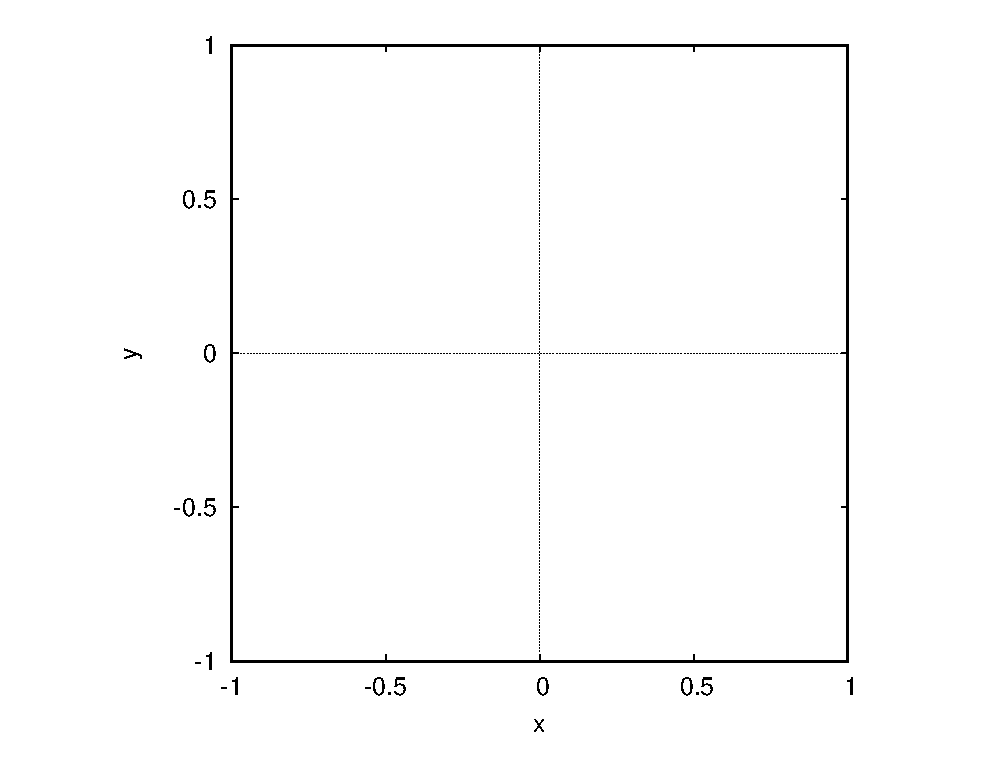
\includegraphics[width=\linewidth, height=30mm]{pic/_old_sol__0_0_1__0__10__1e2_trajectory}
        \caption{Траектория $X, Y$}
        \label{fig:_old_sol__0_0_1__0__10__1e2_trajectory}
    \end{subfigure}
    \begin{subfigure}[t]{0.3\textwidth}
        \centering
        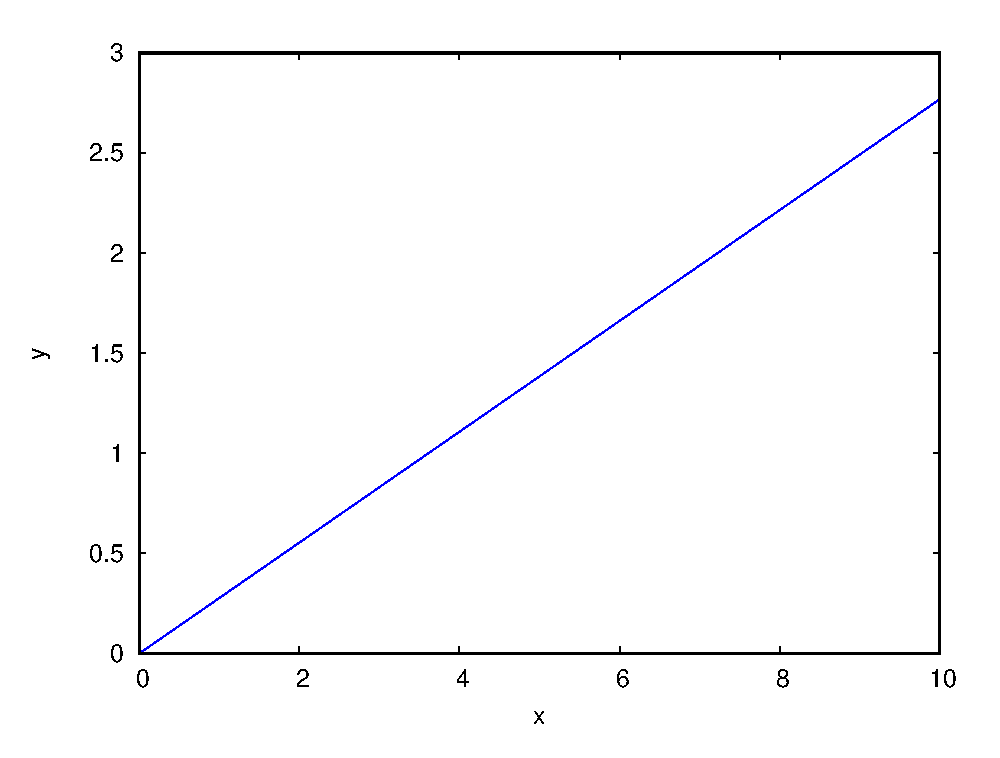
\includegraphics[width=\linewidth, height=30mm]{pic/_old_sol__0_0_1__0__10__1e2_theta}
        \caption{$\theta(t)$}
        \label{fig:_old_sol__0_0_1__0__10__1e2_theta}
    \end{subfigure}
    \vspace{12pt}
    
    \begin{subfigure}[t]{0.3\textwidth}
        \centering
        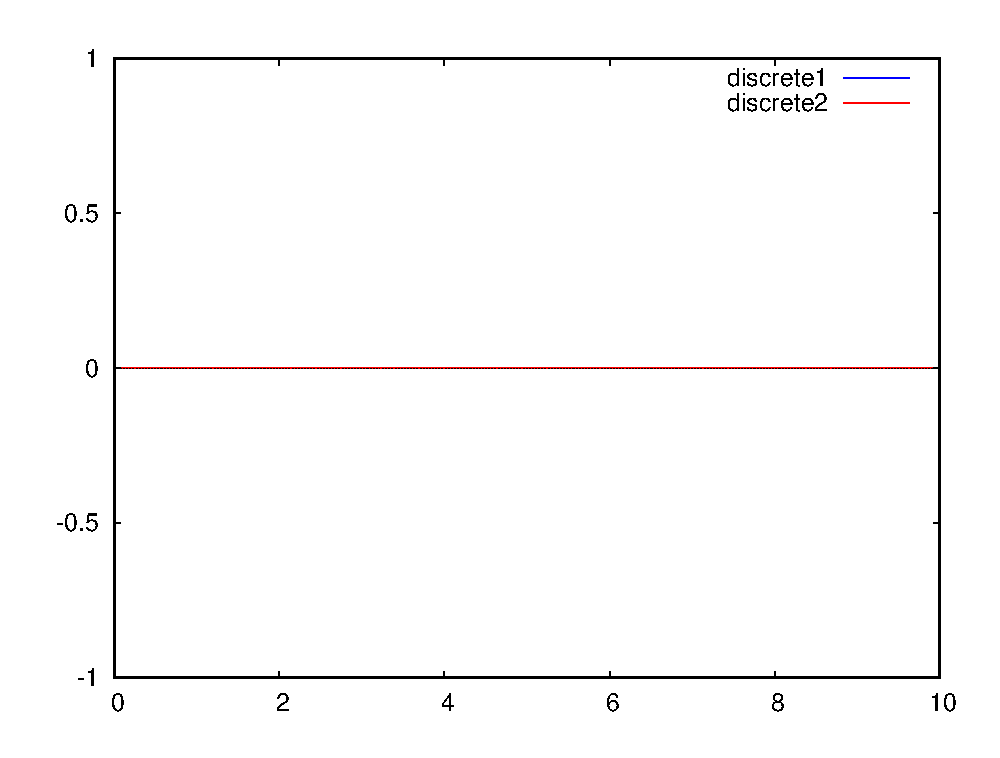
\includegraphics[width=\linewidth, height=30mm]{pic/_old_sol__0_0_1__0__10__1e2_nu12}
        \caption{$\nu_1(t), \nu_2(t)$}
        \label{fig:_old_sol__0_0_1__0__10__1e2_nu12}    
    \end{subfigure}
    \hfill
    \begin{subfigure}[t]{0.3\textwidth}
        \centering
        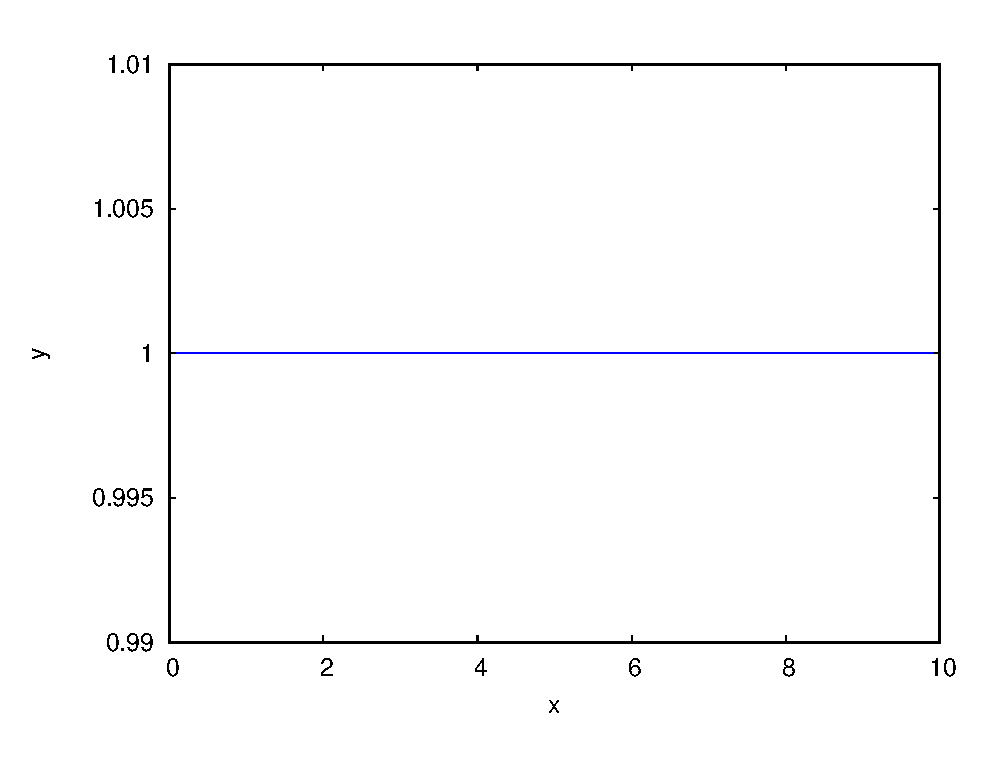
\includegraphics[width=\linewidth, height=30mm]{pic/_old_sol__0_0_1__0__10__1e2_nu3} \\
        \caption{$\nu_3(t)$}
        \label{fig:_old_sol__0_0_1__0__10__1e2_nu3}
    \end{subfigure}
    \hfill
    \begin{subfigure}[t]{0.3\textwidth}
        \centering
        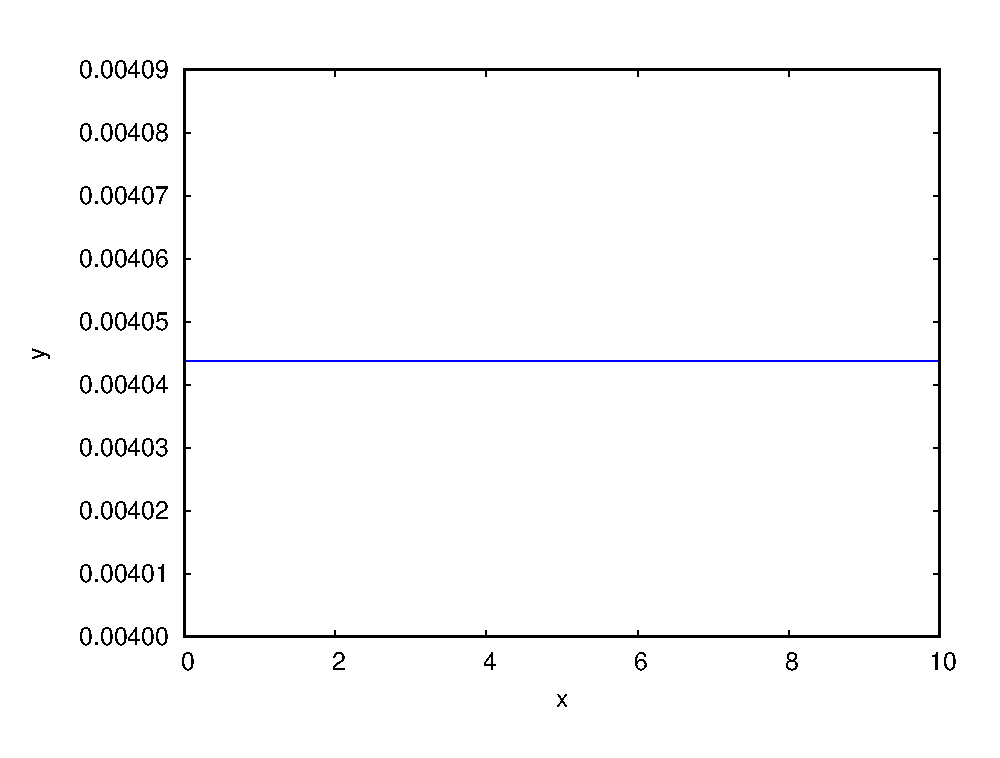
\includegraphics[width=\linewidth, height=30mm]{pic/_old_sol__0_0_1__0__10__1e2_kin_en}
        \caption{Кинетическая энергия}
        \label{fig:_old_sol__0_0_1__0__10__1e2_kin_en}
    \end{subfigure}
    
    \caption{Экипаж без роликов. Вращение вокруг своей оси ($\nu_{1,2}(0) = 0, \nu_3 = 1$). Центр экипажа неподвижен, скорость вращения и энергия постоянны.}
    \label{fig:old_selfrot}
\end{figure}

% \begin{figure}
    \centering

    % \begin{subfigure}[t]{0.3\textwidth}
    %     \centering
    %     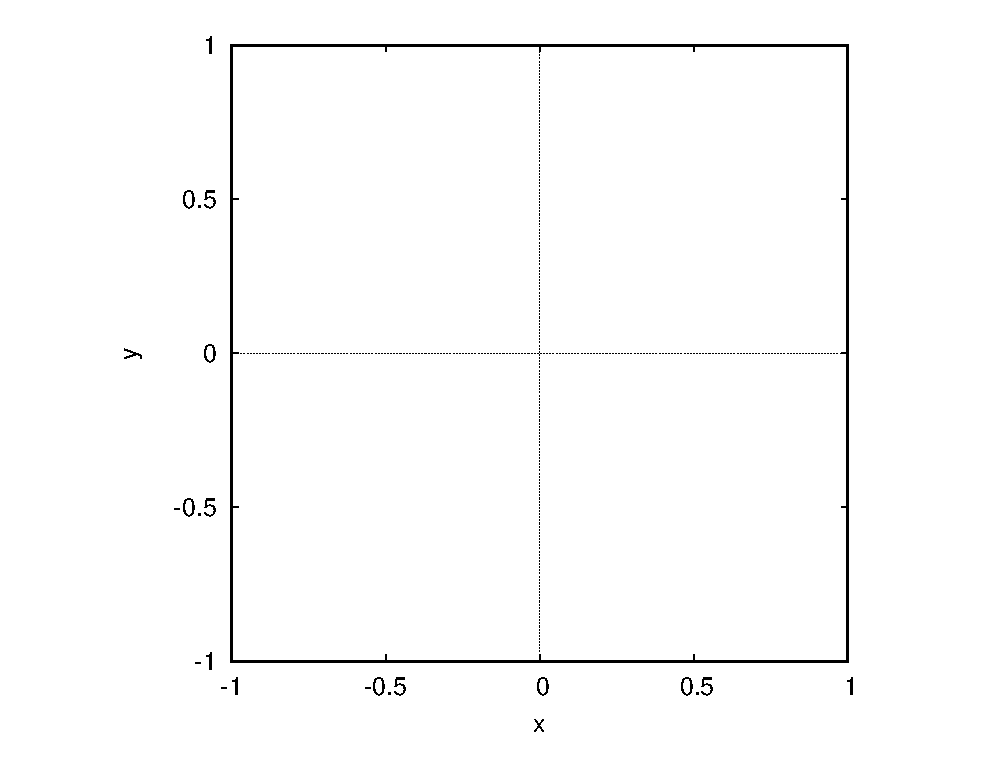
\includegraphics[width=\linewidth, height=30mm]{pic/_sol__0_0_1__0__10__1e2_trajectory}
    %     \caption{Траектория $X, Y$}
    %     \label{fig:_sol__0_0_1__0__10__1e2_trajectory}
    % \end{subfigure}
    % \begin{subfigure}[t]{0.3\textwidth}
    %     \centering
    %     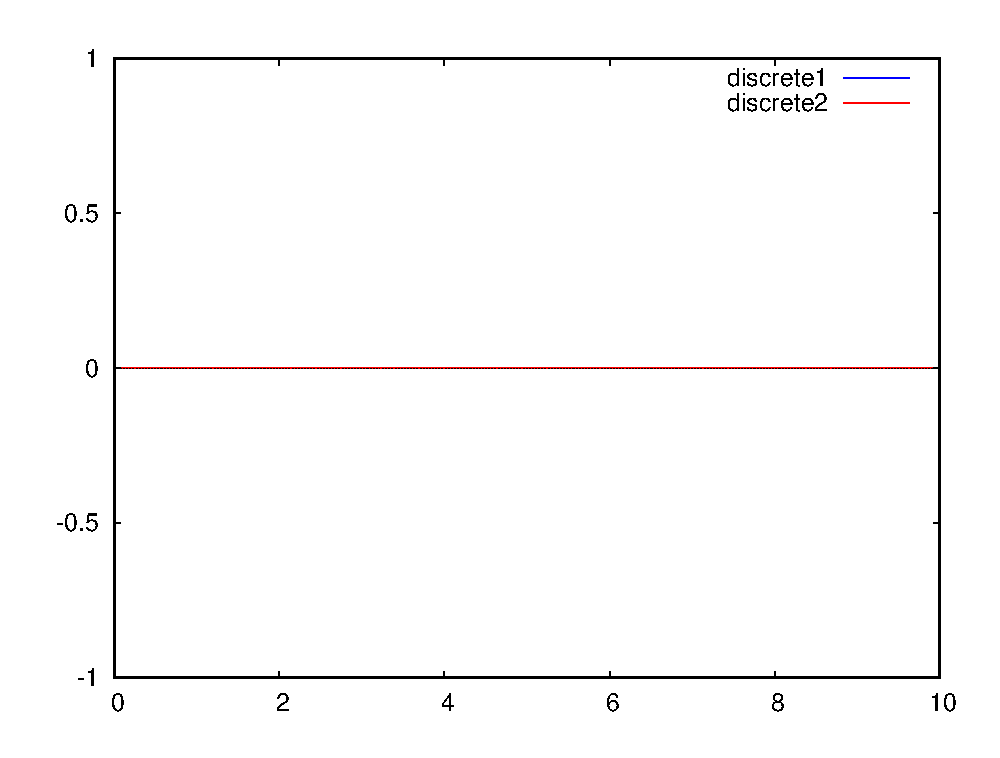
\includegraphics[width=\linewidth, height=30mm]{pic/_sol__0_0_1__0__10__1e2_nu12}
    %     \caption{$\nu_1(t), \nu_2(t)$}
    %     \label{fig:_sol__0_0_1__0__10__1e2_nu12}    
    % \end{subfigure}
    
    % \begin{subfigure}[t]{0.3\textwidth}
    %     \centering
    %     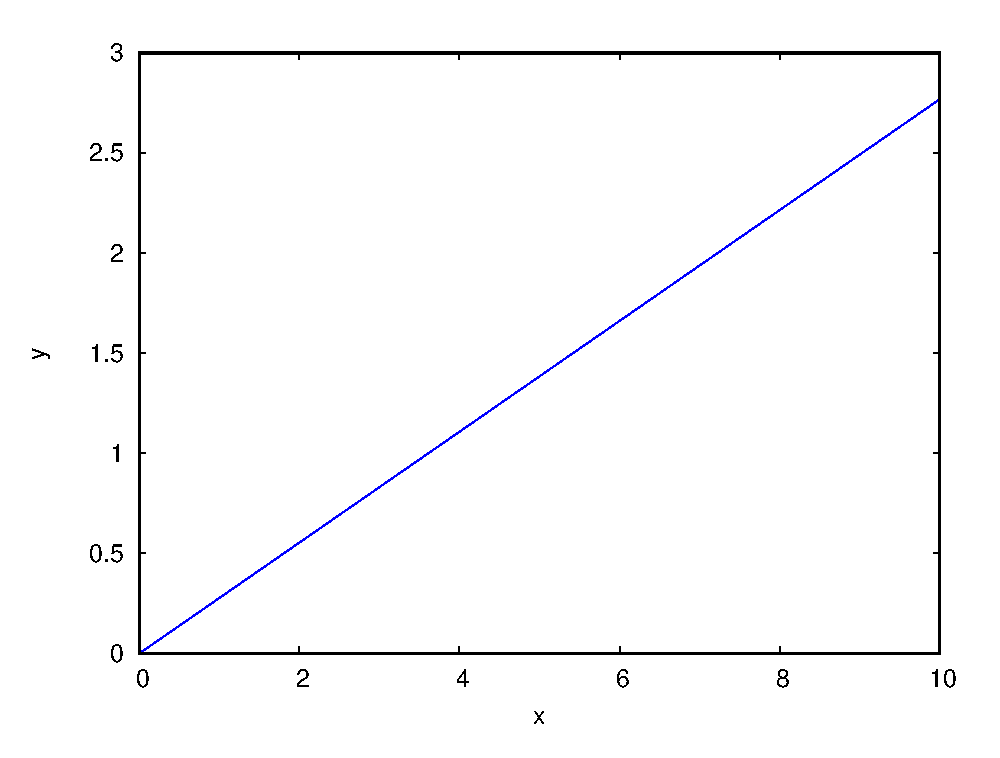
\includegraphics[width=\linewidth, height=30mm]{pic/_sol__0_0_1__0__10__1e2_theta}
    %     \caption{$\theta(t)$}
    %     \label{fig:_sol__0_0_1__0__10__1e2_theta}
    % \end{subfigure}
    % \vspace{12pt}
    
    % \begin{subfigure}[t]{0.3\textwidth}
    %     \centering
    %     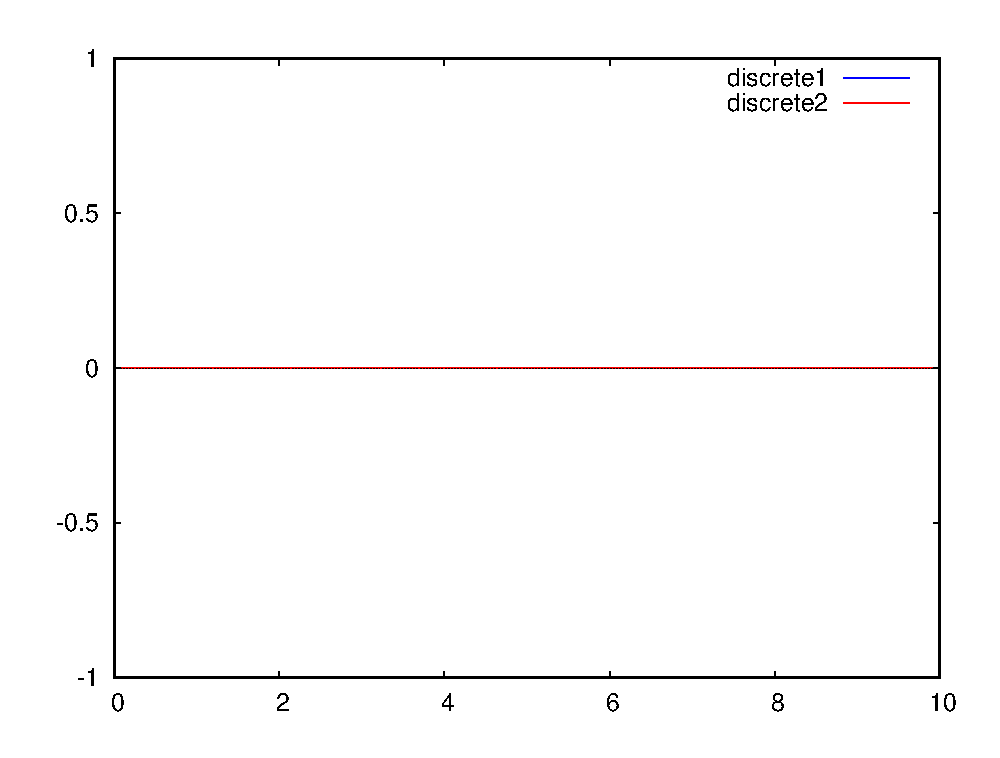
\includegraphics[width=\linewidth, height=30mm]{pic/_sol__0_0_1__0__10__1e2_nu12}
    %     \caption{$\nu_1(t), \nu_2(t)$}
    %     \label{fig:_sol__0_0_1__0__10__1e2_nu12}    
    % \end{subfigure}
    % \hfill
    % \begin{subfigure}[t]{0.3\textwidth}
    %     \centering
    %     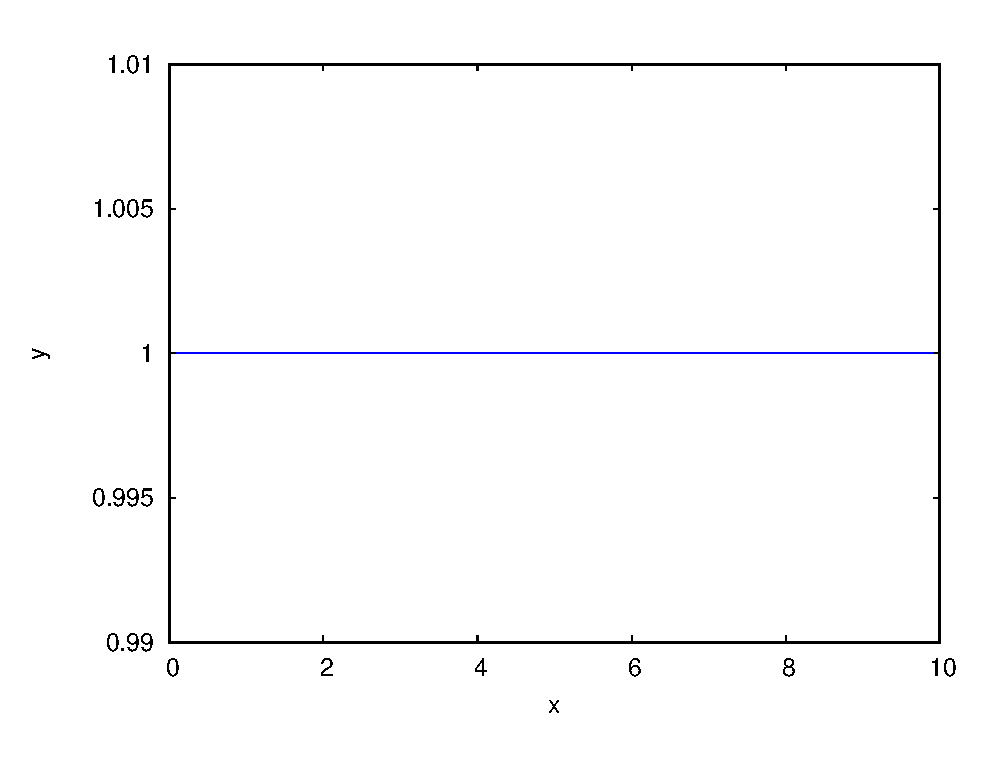
\includegraphics[width=\linewidth, height=30mm]{pic/_sol__0_0_1__0__10__1e2_nu3} \\
    %     \caption{$\nu_3(t)$}
    %     \label{fig:_sol__0_0_1__0__10__1e2_nu3}
    % \end{subfigure}
    % \hfill
    % \begin{subfigure}[t]{0.3\textwidth}
    %     \centering
    %     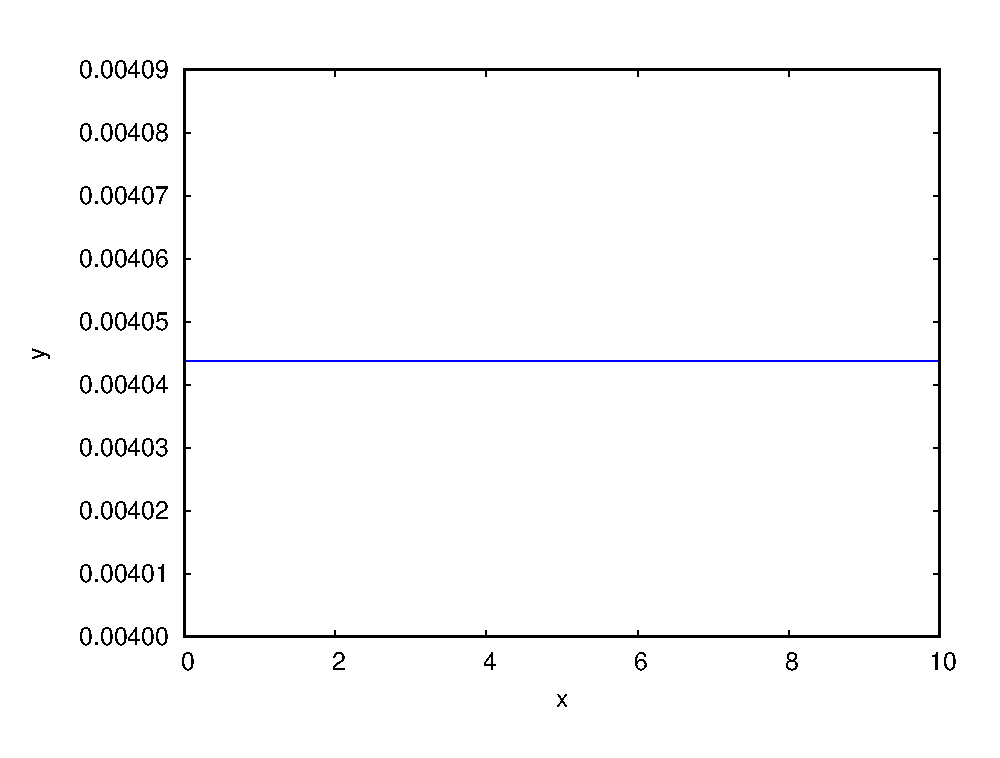
\includegraphics[width=\linewidth, height=30mm]{pic/_sol__0_0_1__0__10__1e2_kin_en}
    %     \caption{Кинетическая энергия}
    %     \label{fig:_sol__0_0_1__0__10__1e2_kin_en}
    % \end{subfigure}
    
    \begin{subfigure}[t]{0.3\textwidth}
        \centering
        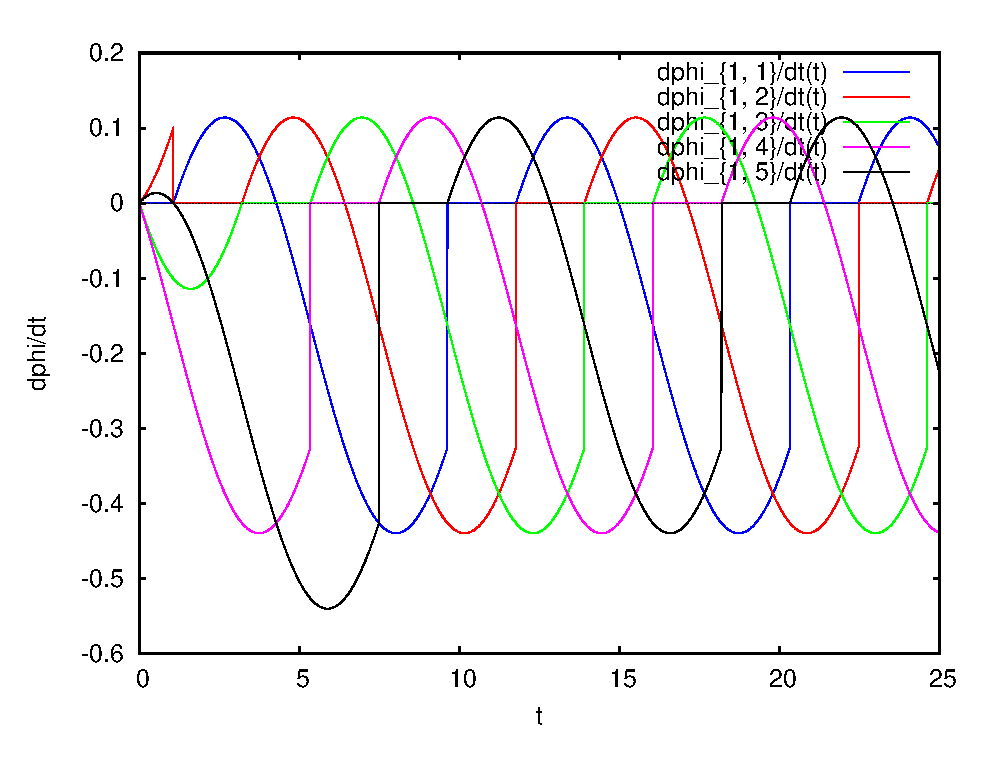
\includegraphics[width=\linewidth]{pic/rol__self_rot__velocities_of_rollers_of_wheel_1}
        \caption{Скорости роликов $\dot{\phi}_{ij}(t)$ на любом колесе}
        \label{fig:rol__self_rot__velocities_of_rollers_of_wheel_1}
    \end{subfigure}
    \begin{subfigure}[t]{0.3\textwidth}
        \centering
        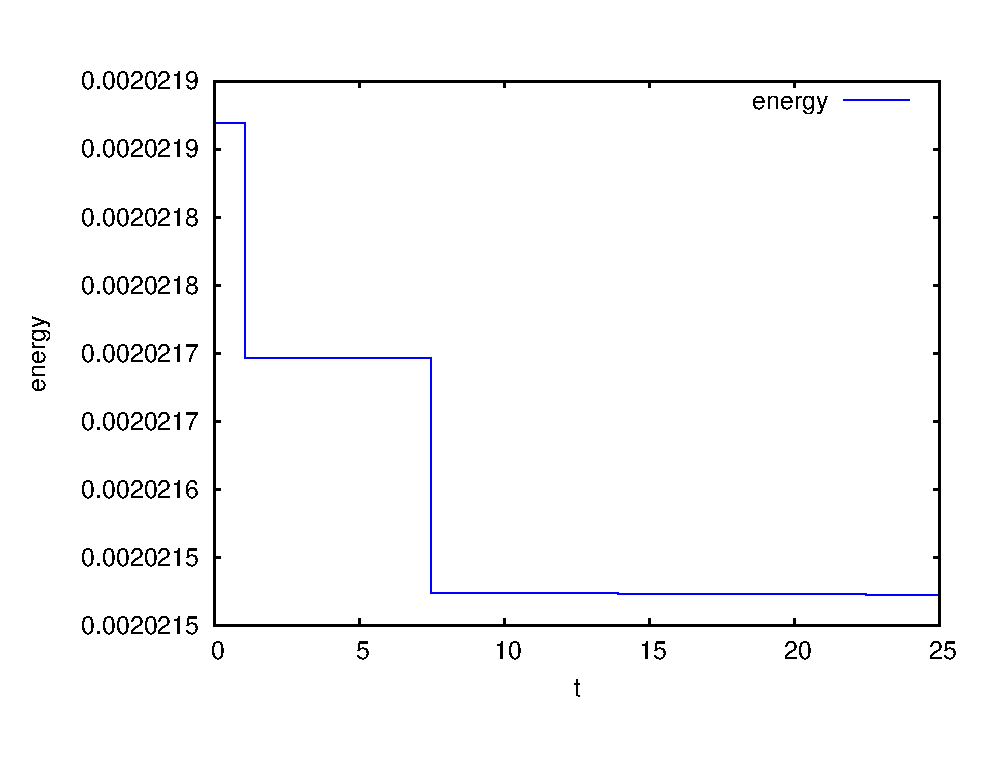
\includegraphics[width=\linewidth]{pic/rol__self_rot__kinetic_energy}
        \caption{Кинетическая энергия}
        \label{fig:rol__self_rot__kinetic_energy}    
    \end{subfigure}
    \begin{subfigure}[t]{0.3\textwidth}
        \centering
        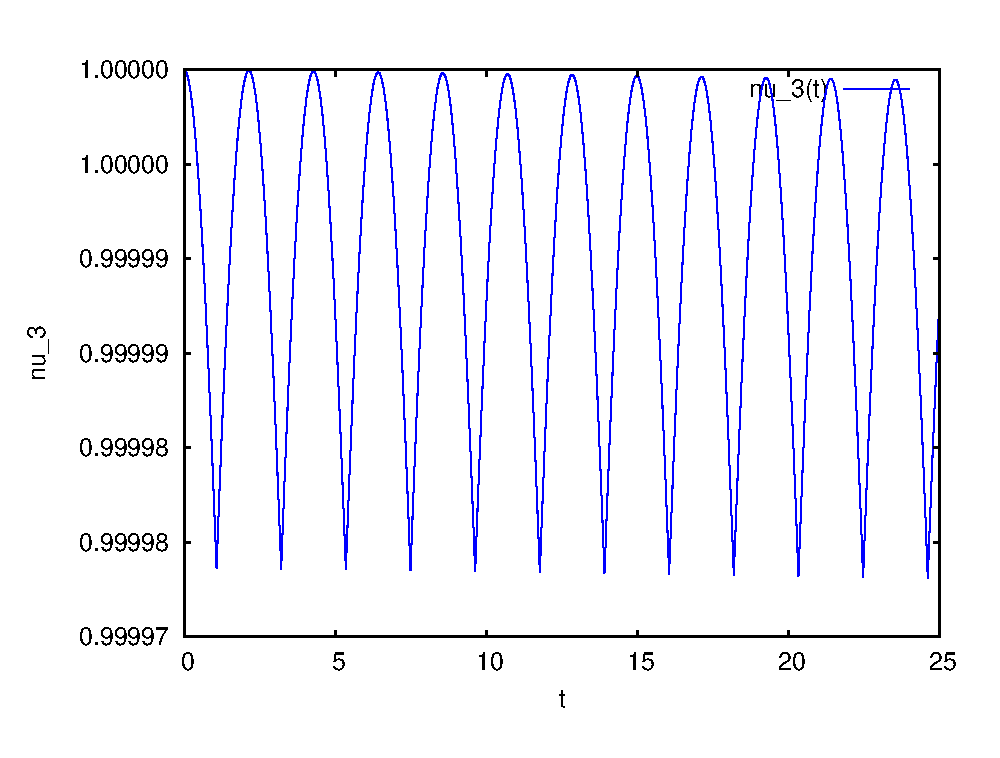
\includegraphics[width=\linewidth]{pic/rol__self_rot__velocity_of_self_rotation}
        \caption{Угловая скорость собственного вращения $\nu_3(t)$}
        \label{fig:rol__self_rot__velocity_of_self_rotation}    
    \end{subfigure}

    \caption{Экипаж с роликами. Вращение вокруг своей оси ($\nu_{1,2}(0) = 0, \nu_3 = 1$).}
    \label{fig:selfrot}
    
\end{figure}


% \begin{figure}
    \centering
    \begin{subfigure}[t]{0.3\textwidth}
        \centering
        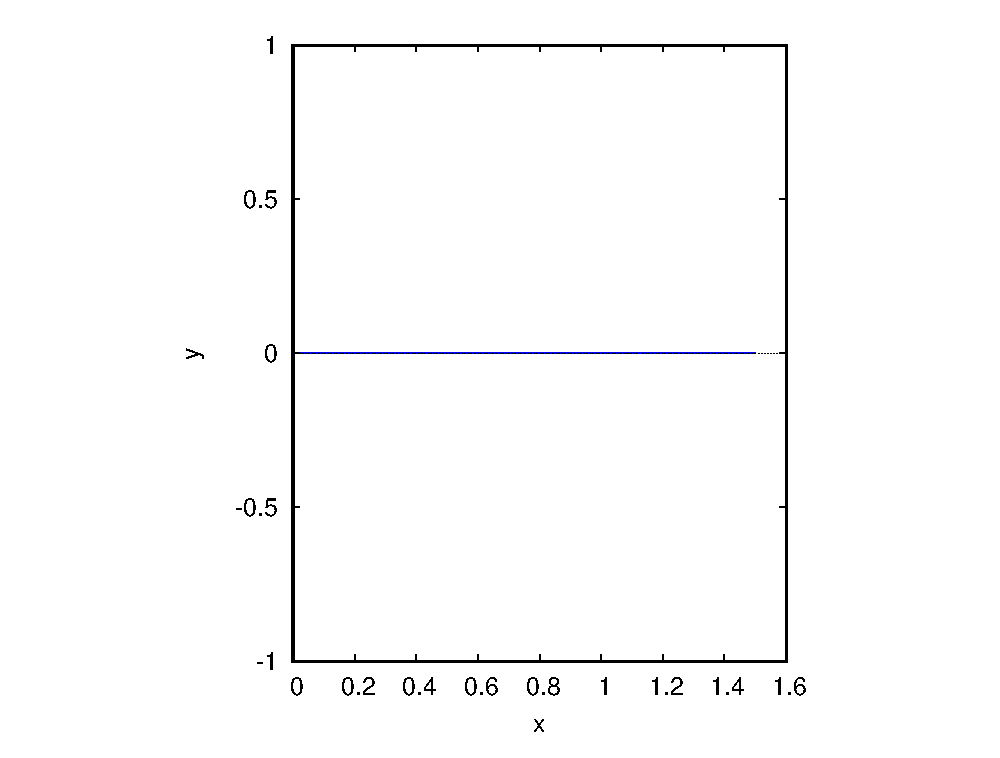
\includegraphics[width=\linewidth, height=30mm]{pic/_old_sol__1_0_0__0__10__1e2_trajectory}
        \caption{Траектория $X, Y$}
        \label{fig:_old_sol__1_0_0__0__10__1e2_trajectory}
    \end{subfigure}
    \begin{subfigure}[t]{0.3\textwidth}
        \centering
        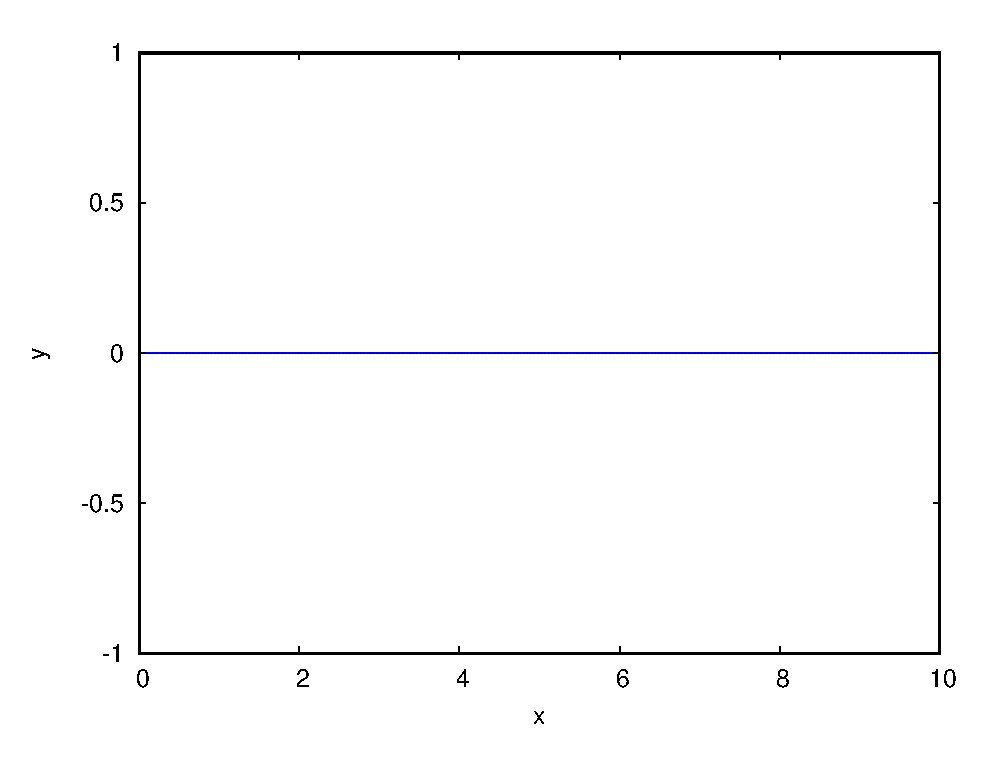
\includegraphics[width=\linewidth, height=30mm]{pic/_old_sol__1_0_0__0__10__1e2_theta}
        \caption{$\theta(t)$}
        \label{fig:_old_sol__1_0_0__0__10__1e2_theta}
    \end{subfigure}
    \vspace{12pt}
    
    \begin{subfigure}[t]{0.3\textwidth}
        \centering
        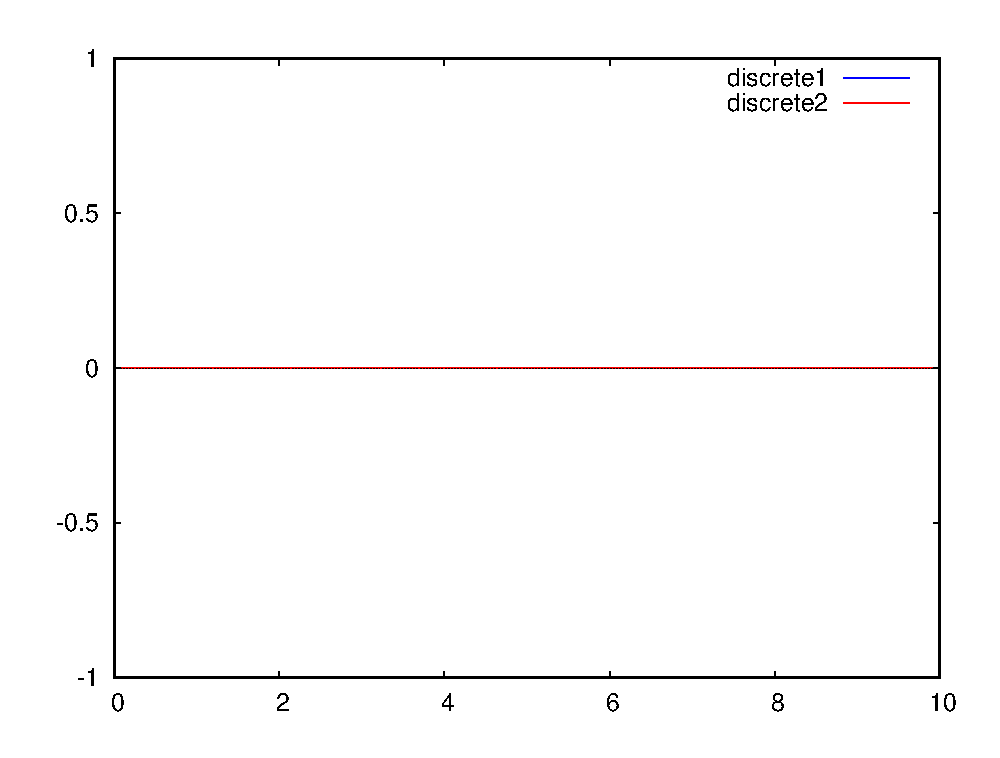
\includegraphics[width=\linewidth, height=30mm]{pic/_old_sol__1_0_0__0__10__1e2_nu12_centered}
        \caption{$\nu_1(t), \nu_2(t)$}
        \label{fig:_old_sol__1_0_0__0__10__1e2_nu12_centered}    
    \end{subfigure}
    \hfill
    \begin{subfigure}[t]{0.3\textwidth}
        \centering
        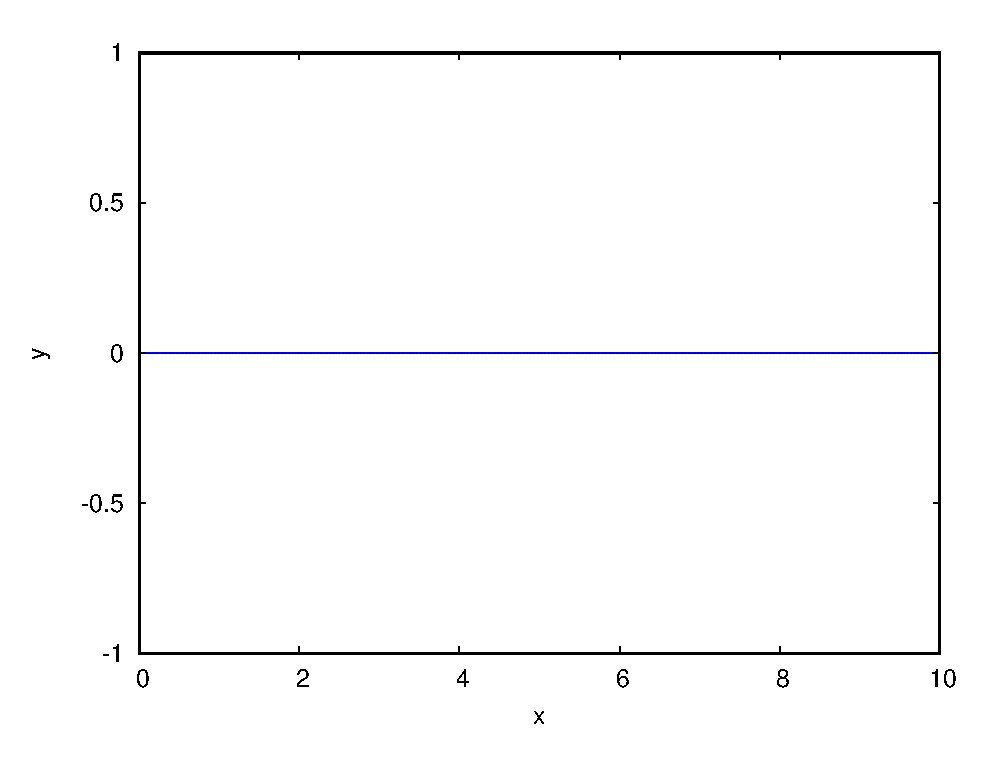
\includegraphics[width=\linewidth, height=30mm]{pic/_old_sol__1_0_0__0__10__1e2_nu3} \\
        \caption{$\nu_3(t)$}
        \label{fig:_old_sol__1_0_0__0__10__1e2_nu3}
    \end{subfigure}
    \hfill
    \begin{subfigure}[t]{0.3\textwidth}
        \centering
        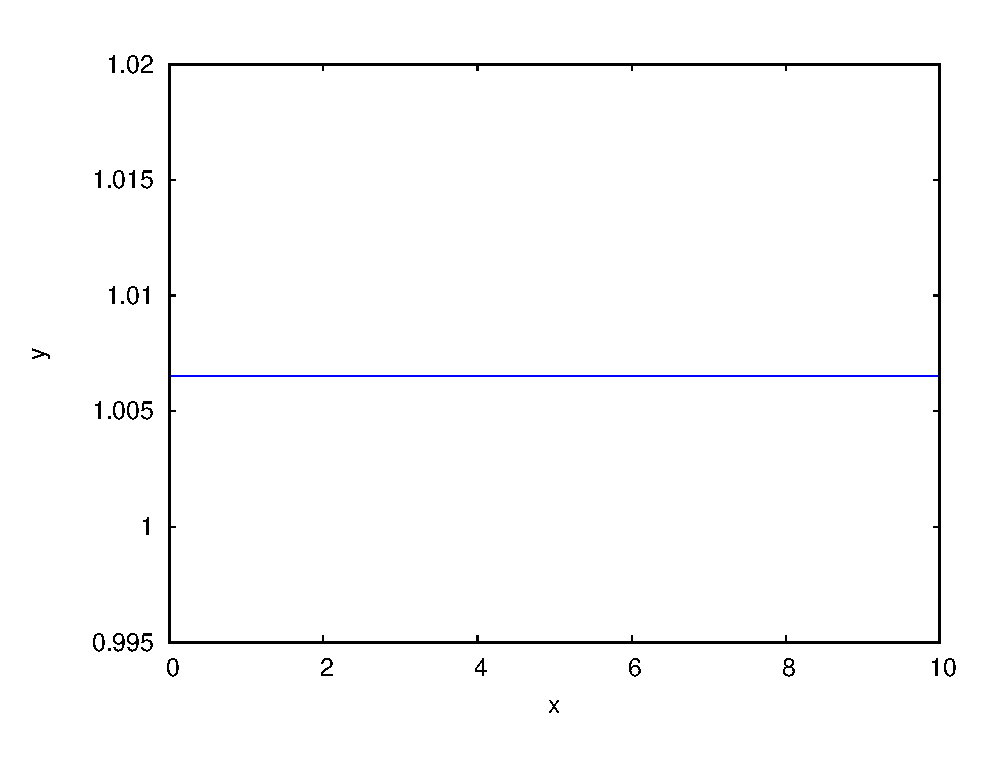
\includegraphics[width=\linewidth, height=30mm]{pic/_old_sol__1_0_0__0__10__1e2_kin_en}
        \caption{Кинетическая энергия}
        \label{fig:_old_sol__1_0_0__0__10__1e2_kin_en}
    \end{subfigure}
    
    \caption{Экипаж без роликов. Движение по прямой ($\nu_1(0) = 1, \nu_{2,3} = 0$). Экипаж равномерно движется по прямой, не вращаясь, энергия постоянна.}
    \label{fig:old_straight}
\end{figure}


% \begin{figure}[H]
    \centering

    \begin{columns}
        \column{0.45\textwidth}
            \centering
            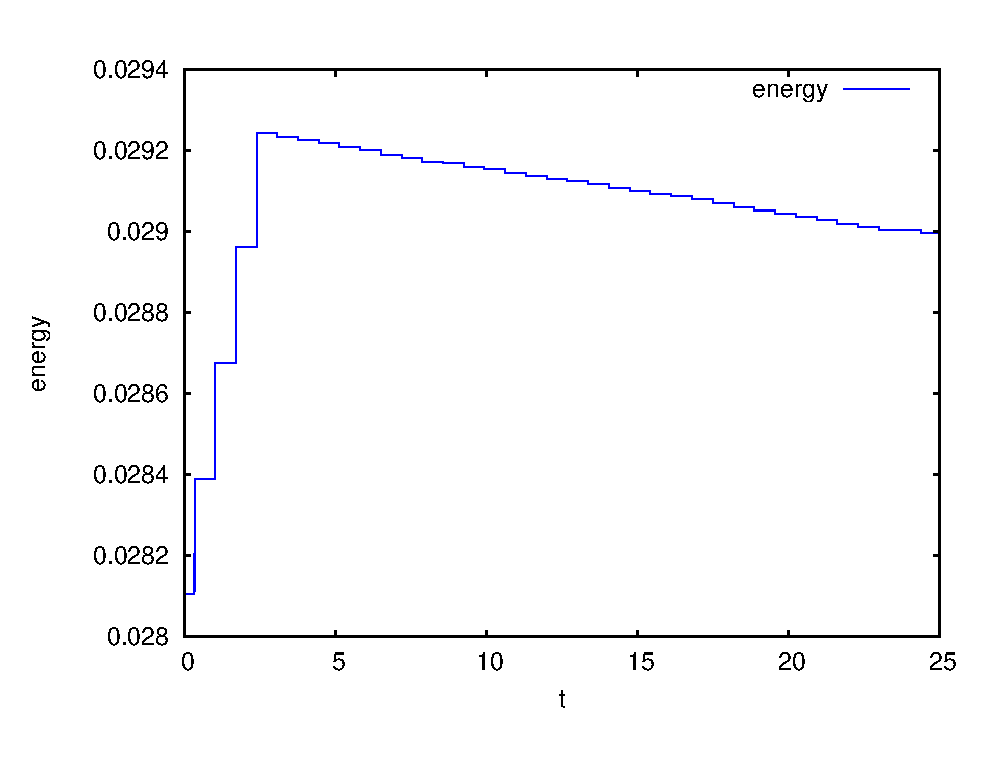
\includegraphics[width=\linewidth]{pic/rol__straight__kinetic_energy}\\
            Кинетическая энергия
        \column{0.45\textwidth}
            \centering
            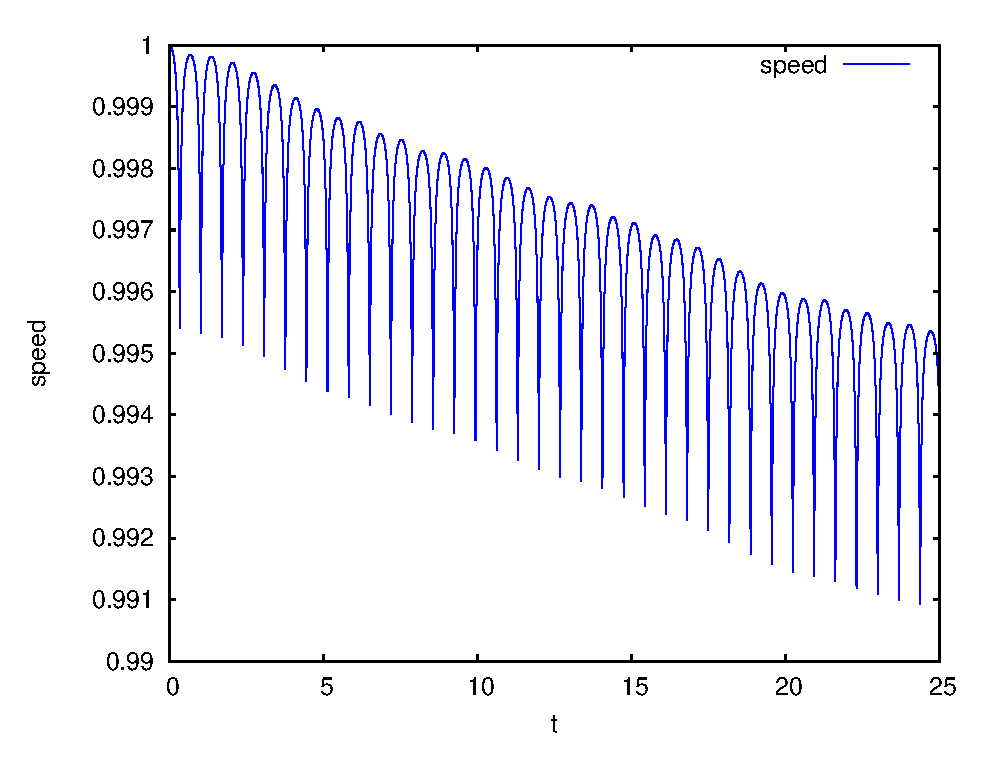
\includegraphics[width=\linewidth]{pic/rol__straight__speed_of_center_of_mass}\\
            Скорость центра масс
    \end{columns}
    
    \begin{columns}
        \column{0.35\textwidth}
            \centering
            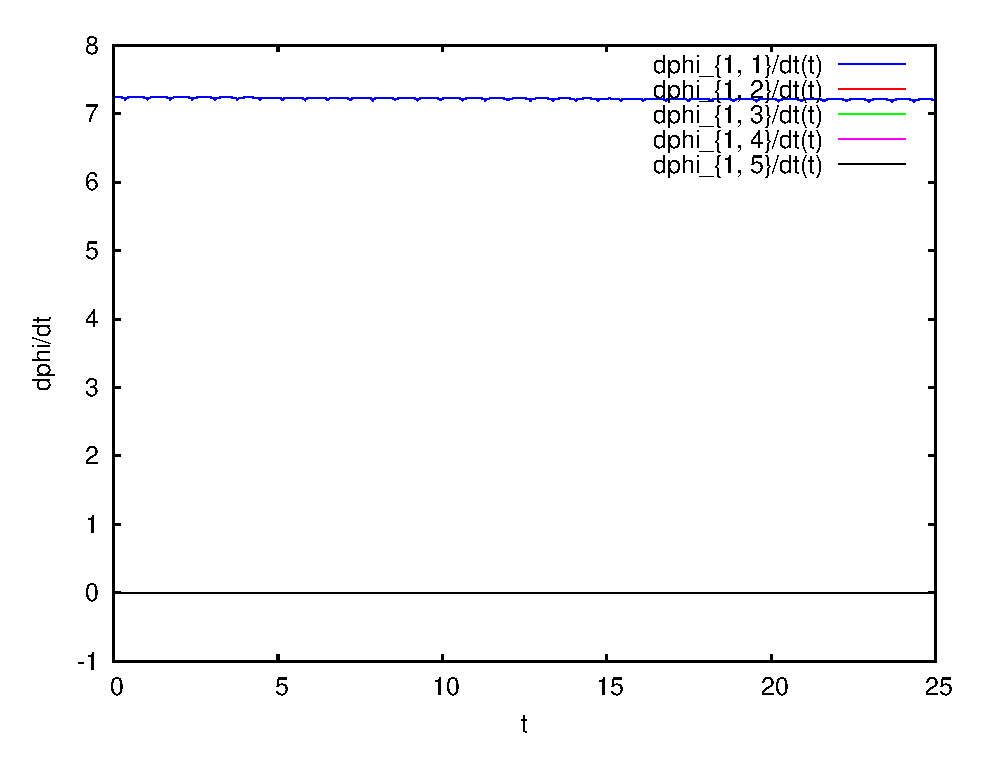
\includegraphics[width=\linewidth]{pic/rol__straight__velocities_of_rollers_of_wheel_1}\\
            $\dot{\phi}_{ij}(t)$ на переднем колесе
        \column{0.45\textwidth}
            \centering
            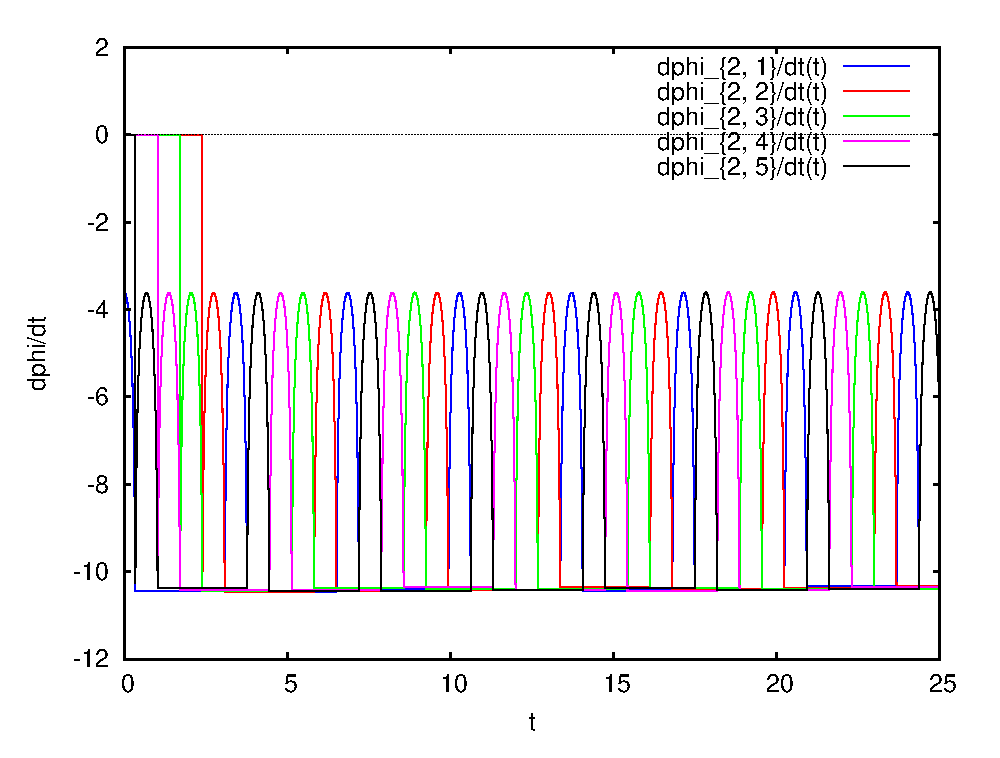
\includegraphics[width=\linewidth]{pic/rol__straight__velocities_of_rollers_of_wheel_2}\\
            $\dot{\phi}_{ij}(t)$ на правом заднем колесе
    \end{columns}

\end{figure}


%\section{Результаты расчетов}

\newpage

{\bf Фигуры.}
\stepcounter{section}

\begin{figure}[H]
    \hspace{-0.6cm}
    \scalebox{1.5}{\asyinclude{./asy/pic_wheel.asy}}
    \quad
    \scalebox{1.5}{\asyinclude{./asy/pic_cart.asy}}
    \caption{\ }
    \label{fig:wheel}
\end{figure}

\begin{figure}[H]
    \centering
    \scalebox{1.5}{\asyinclude{./asy/pic_overlap.asy}}
    \quad
    \scalebox{1.5}{\asyinclude{./asy/pic_change.asy}}
    \caption{\ }
    \label{fig:overlap_and_change}
\end{figure}

% \begin{figure}[H]
    \hspace{-15pt}
    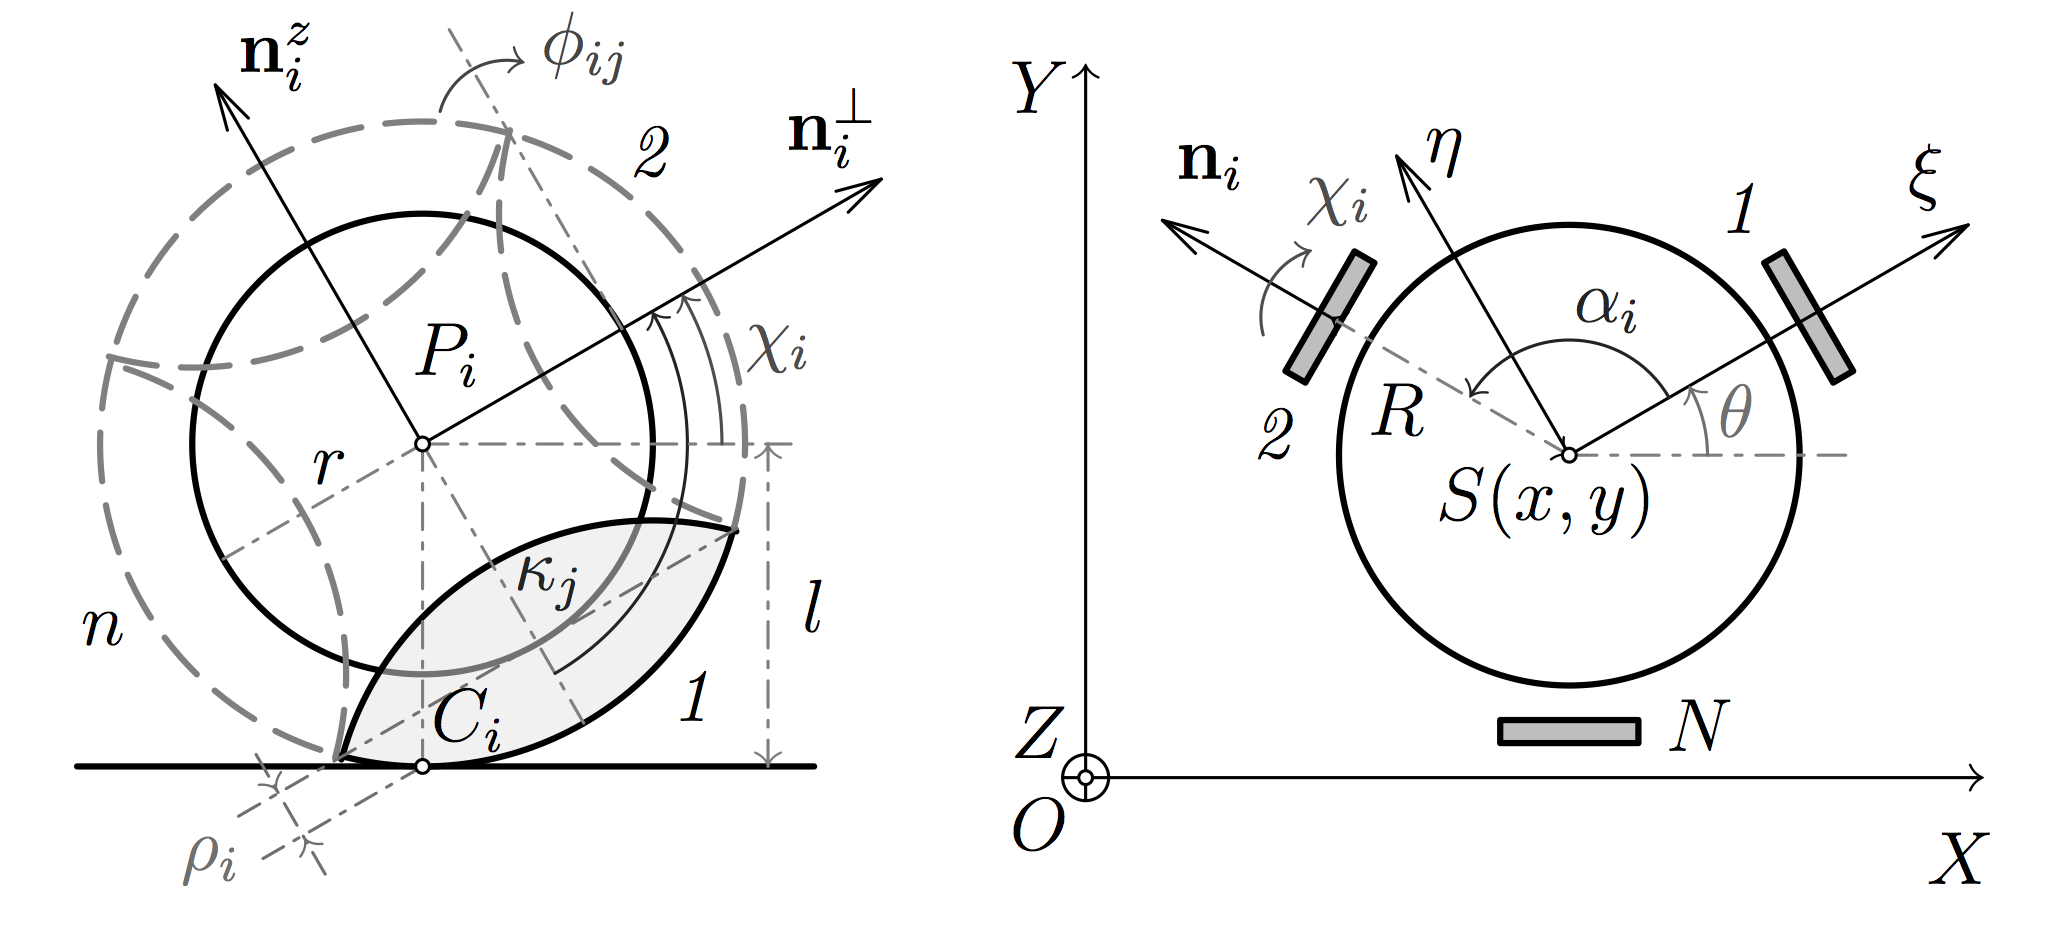
\includegraphics[scale=0.25]{./pic/pic_wheel_cart_300.png}
    \caption{\ }
    \label{fig:wheel}
\end{figure}

\begin{figure}[H]
    \hspace{25pt}
    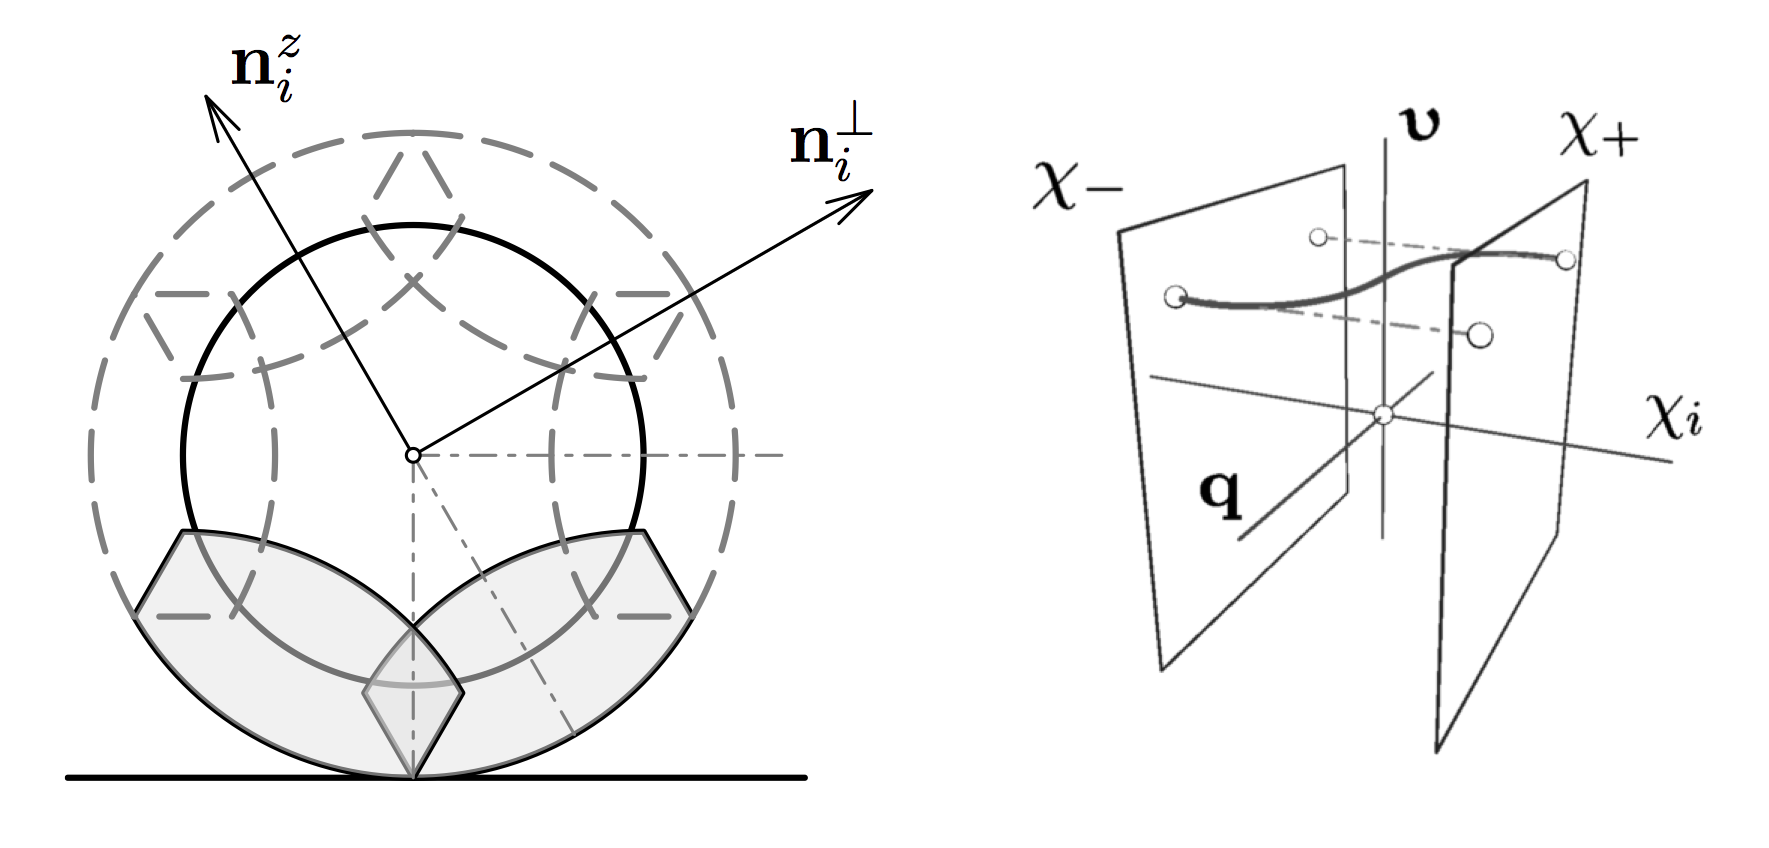
\includegraphics[scale=0.25]{./pic/pic_overlap_change_300.png}
    \caption{\ }
    \label{fig:overlap_and_change}
\end{figure}



\begin{figure}[H]
  \hspace{2.73cm}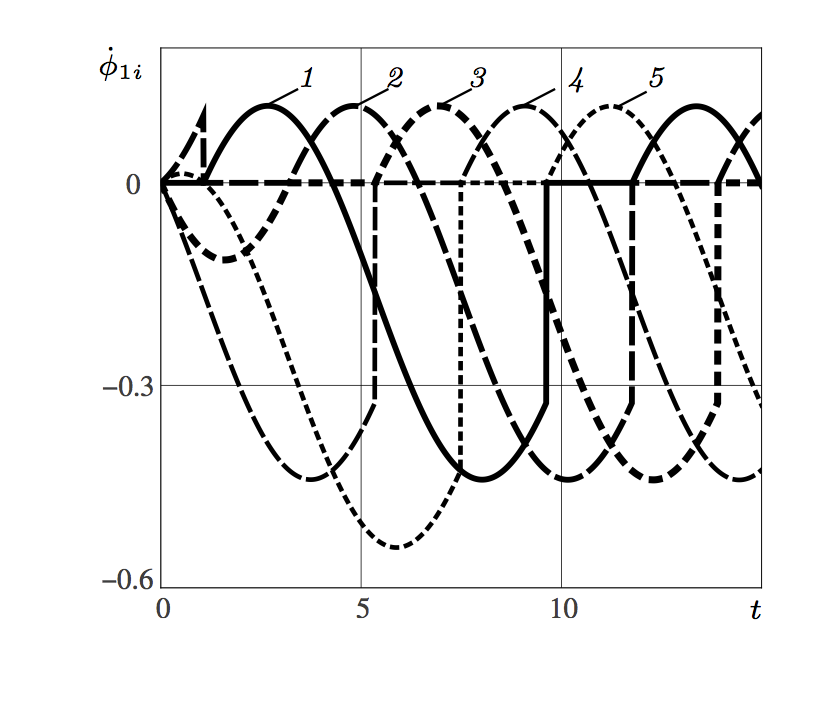
\includegraphics[width=0.6\textwidth]{pic/figure5_1.png}
  \caption{\ }
  %\caption{Угловые скорости роликов колеса при вращении экипажа вокруг вертикали}
  \label{fig:selfrot}
\end{figure}

\begin{figure}[H]
    \minipage{0.45\textwidth}
        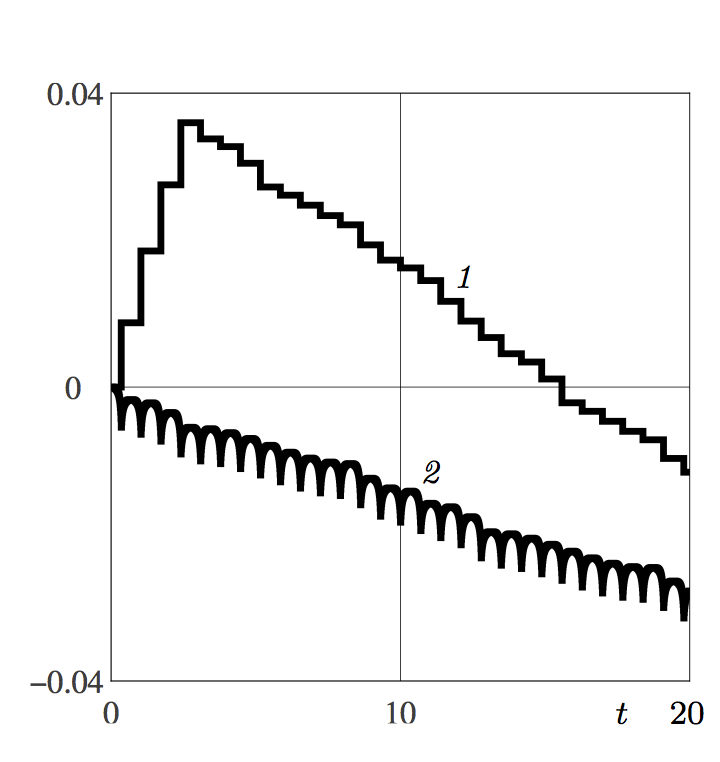
\includegraphics[scale=1.33]{pic/figure6_1.png}
    \endminipage
    \quad
    \minipage{0.45\textwidth}
        \vspace{26pt}
        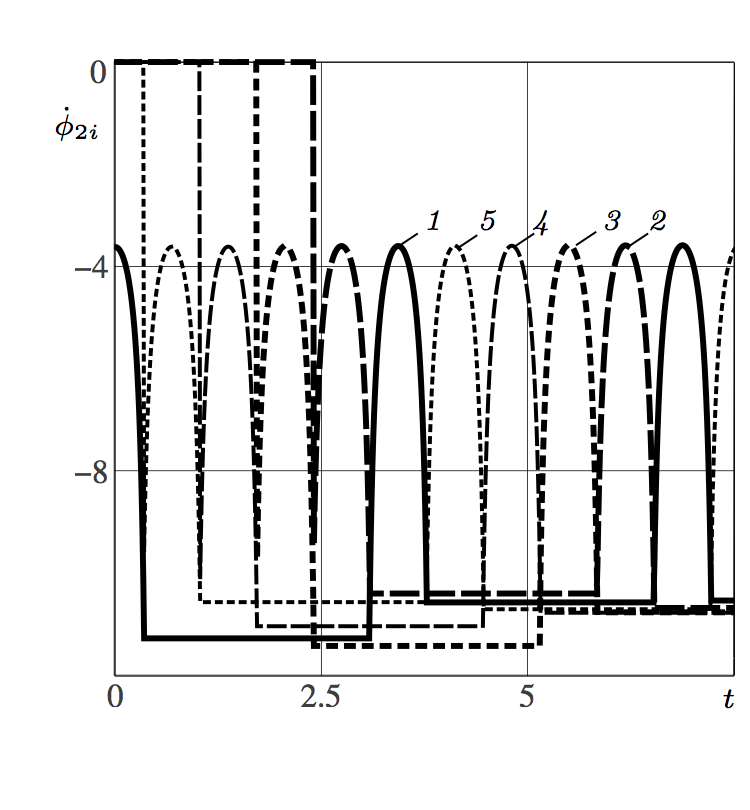
\includegraphics[scale=1.28]{pic/figure6_2.png}
    \endminipage
%\caption{Изменение энергии и скорости центра масс (слева) и угловые скорости роликов бокового колеса (справа) при прямолинейном движении}
  \caption{\ }
  \label{fig:straight}
\end{figure}

% \begin{figure}[H]
%   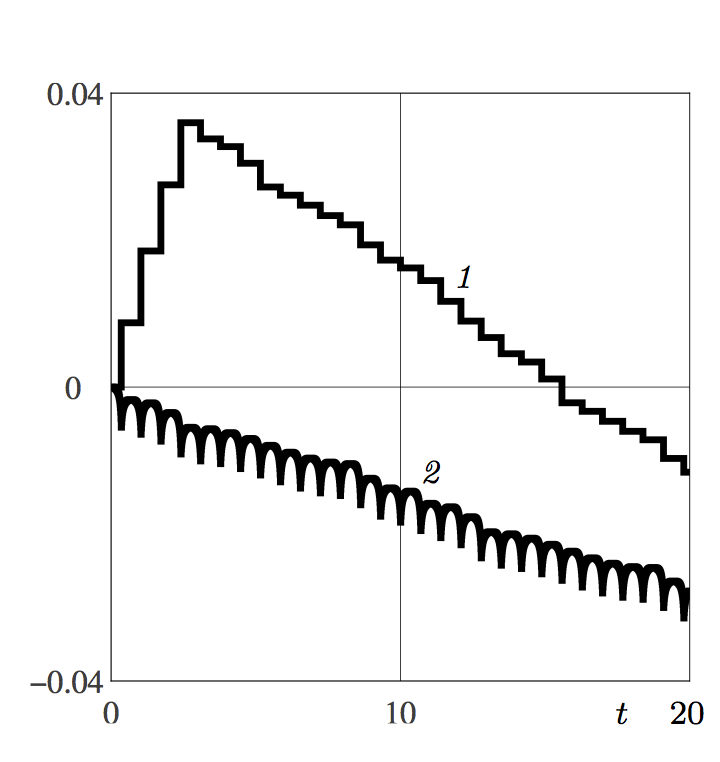
\includegraphics[width=0.45\textwidth]{pic/figure6_1.png}
%   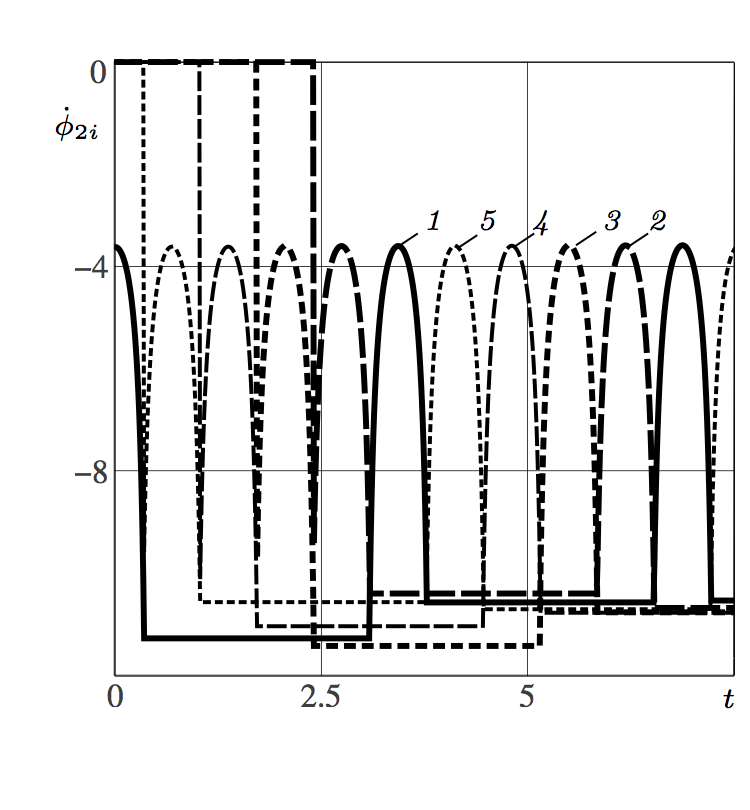
\includegraphics[width=0.45\textwidth]{pic/figure6_2.png}
%   %\caption{Изменение энергии и скорости центра масс (слева) и угловые скорости роликов бокового колеса (справа) при прямолинейном движении}
%   \caption{\ }
%   \label{fig:straight}
% \end{figure}

\begin{figure}[H]
    \hspace{-20pt}
    \minipage{0.5\textwidth}
        \vspace{10pt}
        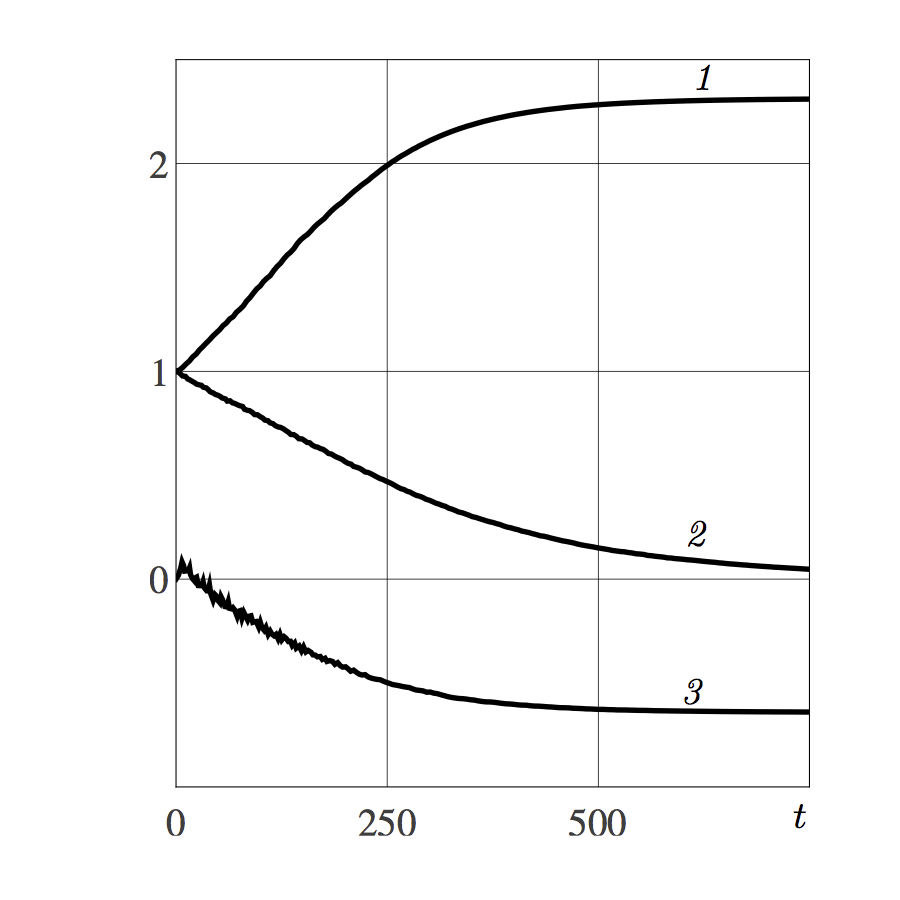
\includegraphics[scale=1.2]{pic/figure7_1.png}
    \endminipage
    \minipage{0.5\textwidth}
        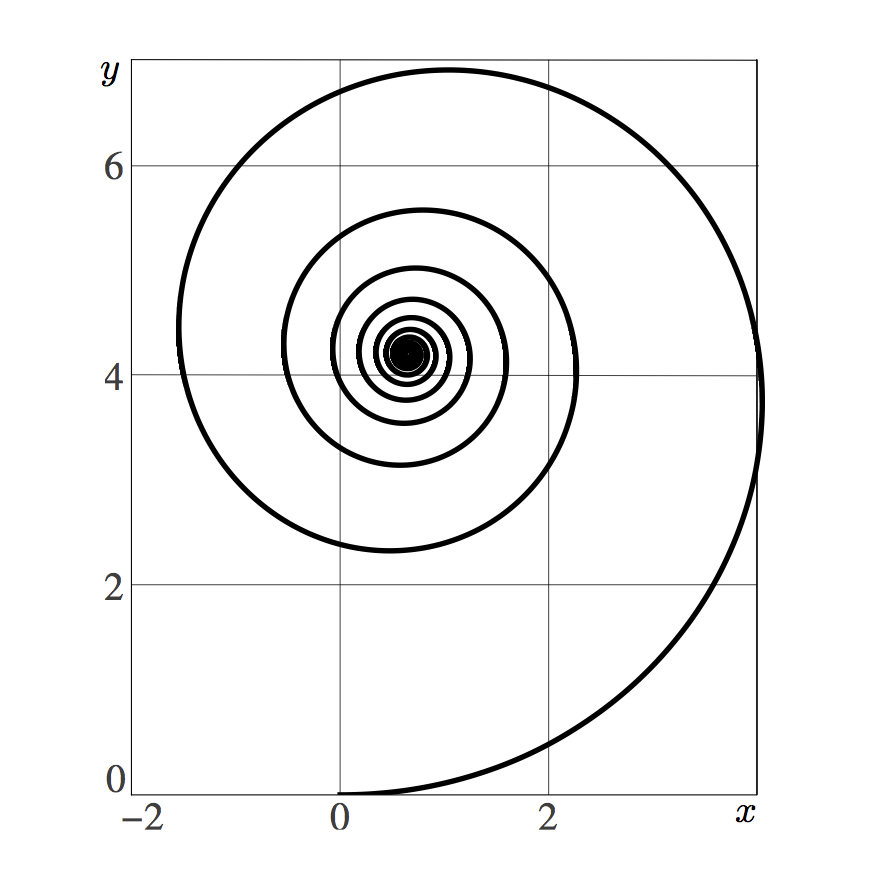
\includegraphics[scale=1.2]{pic/figure7_3.png}
    \endminipage
\end{figure}

\begin{figure}[H]
%   \hspace{-1.4cm}
%   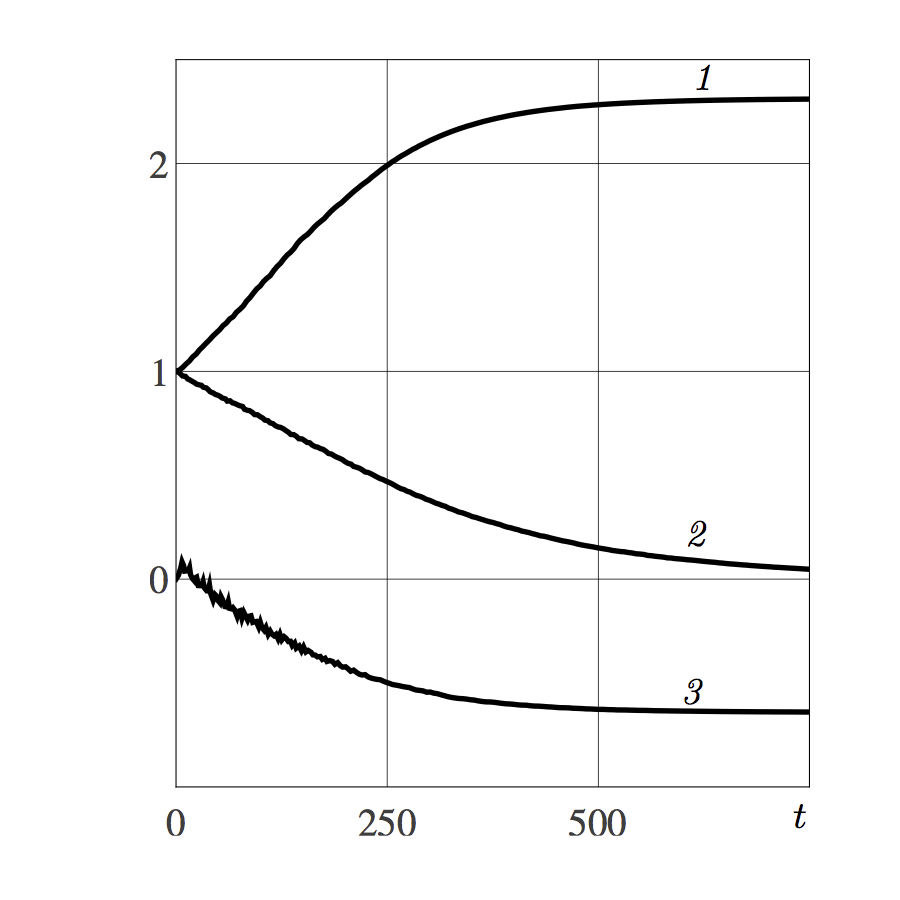
\includegraphics[width=0.6\textwidth]{pic/figure7_1.png}
%   \hspace{-0.7cm}
%   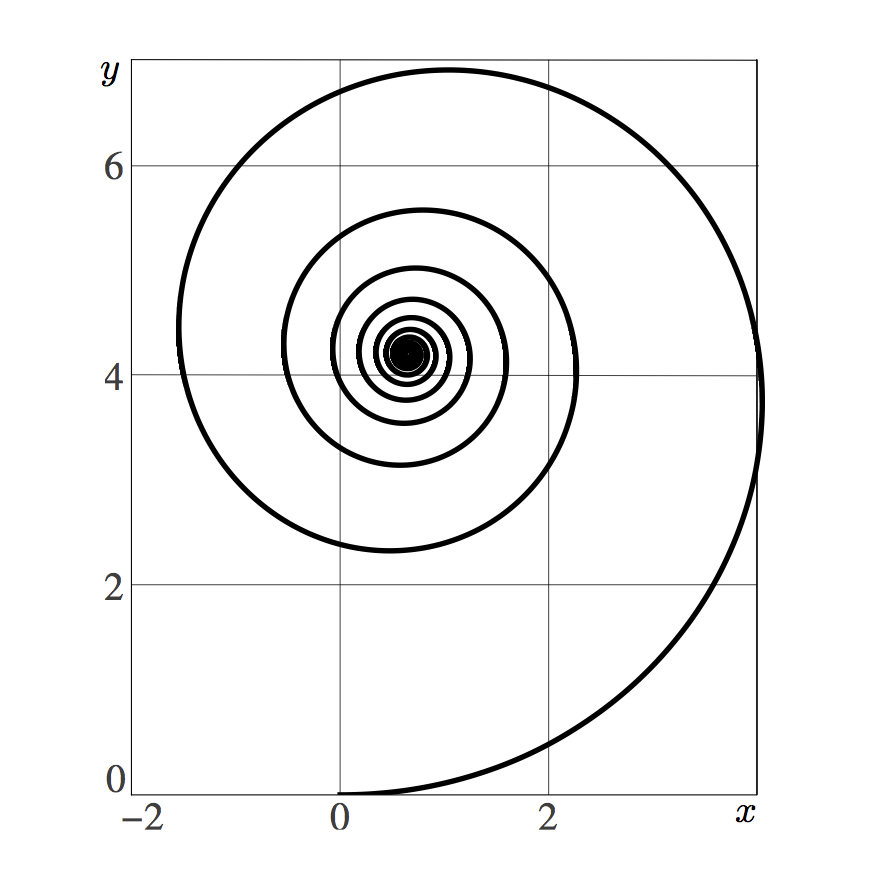
\includegraphics[width=0.59\textwidth]{pic/figure7_3.png}
  \hspace{-14.3pt}
  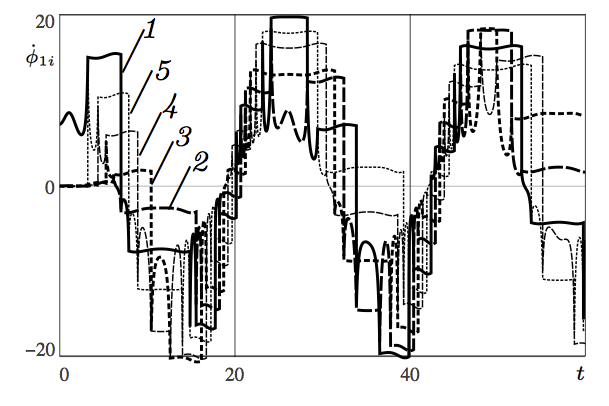
\includegraphics[width=0.9755\textwidth]{pic/figure7_2.png}
  %\caption{Угловая скорость, скорость центра масс и изменение энергии (вверху слева), угловые скорости роликов первого колеса (вверху справа) и траектория центра масс (внизу) при поступательно-вращательном движении}
  \caption{\ }
  \label{fig:wrench}
\end{figure}


%\begin{figure}
    \centering

    % \begin{subfigure}[t]{0.3\textwidth}
    %     \centering
    %     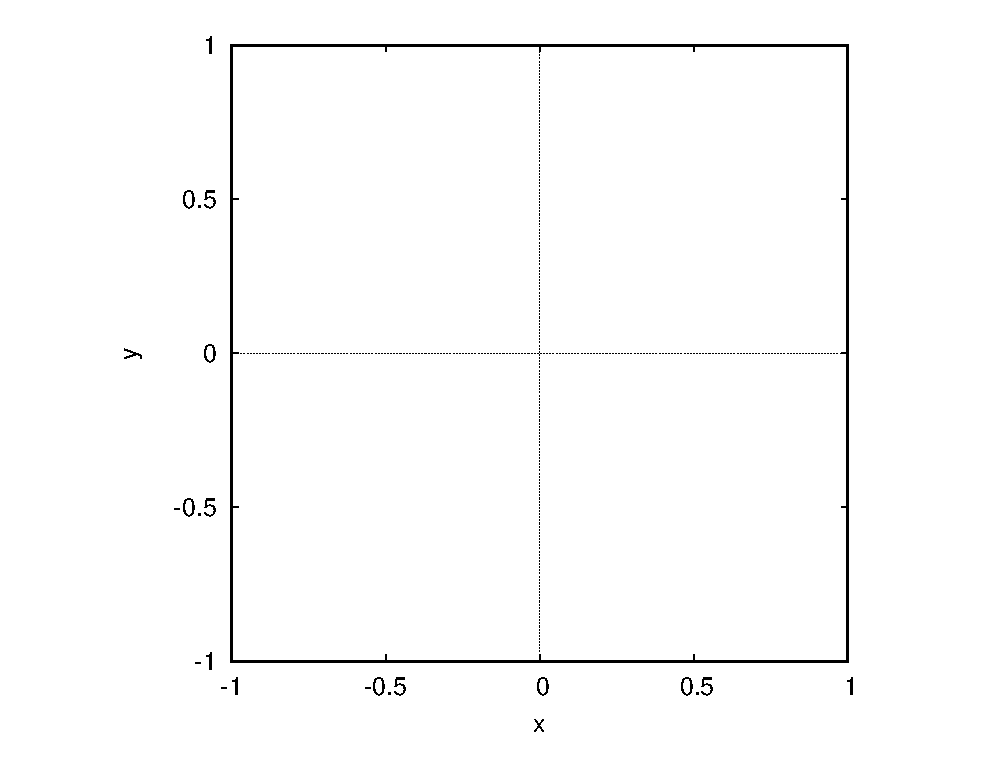
\includegraphics[width=\linewidth, height=30mm]{pic/_sol__0_0_1__0__10__1e2_trajectory}
    %     \caption{Траектория $X, Y$}
    %     \label{fig:_sol__0_0_1__0__10__1e2_trajectory}
    % \end{subfigure}
    % \begin{subfigure}[t]{0.3\textwidth}
    %     \centering
    %     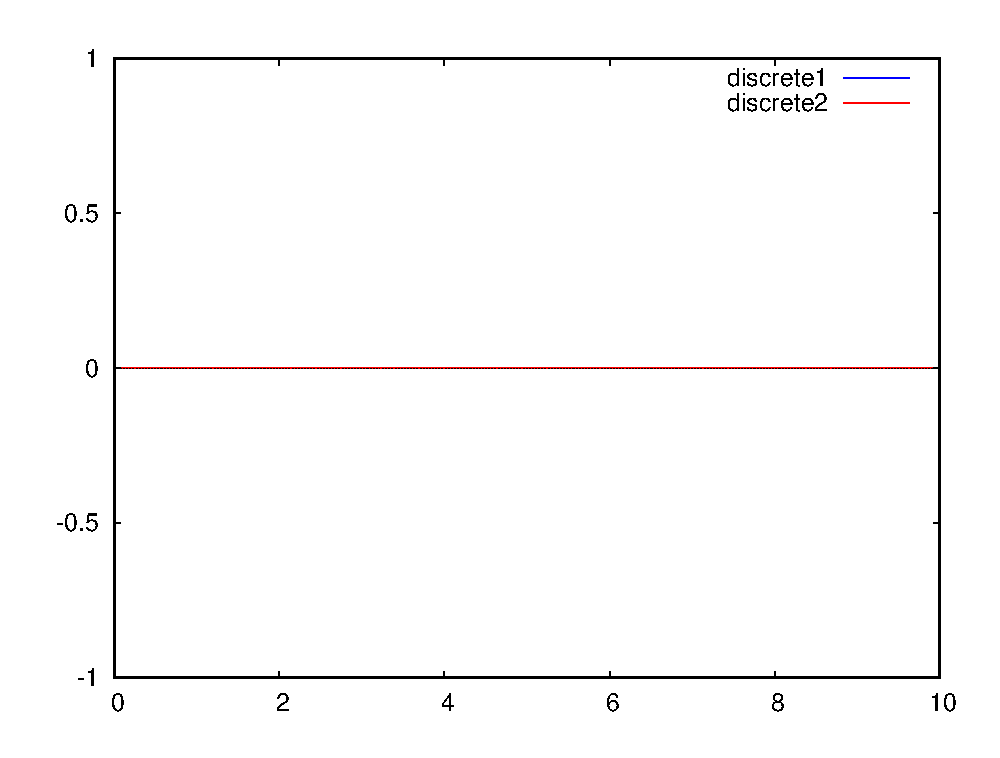
\includegraphics[width=\linewidth, height=30mm]{pic/_sol__0_0_1__0__10__1e2_nu12}
    %     \caption{$\nu_1(t), \nu_2(t)$}
    %     \label{fig:_sol__0_0_1__0__10__1e2_nu12}    
    % \end{subfigure}
    
    % \begin{subfigure}[t]{0.3\textwidth}
    %     \centering
    %     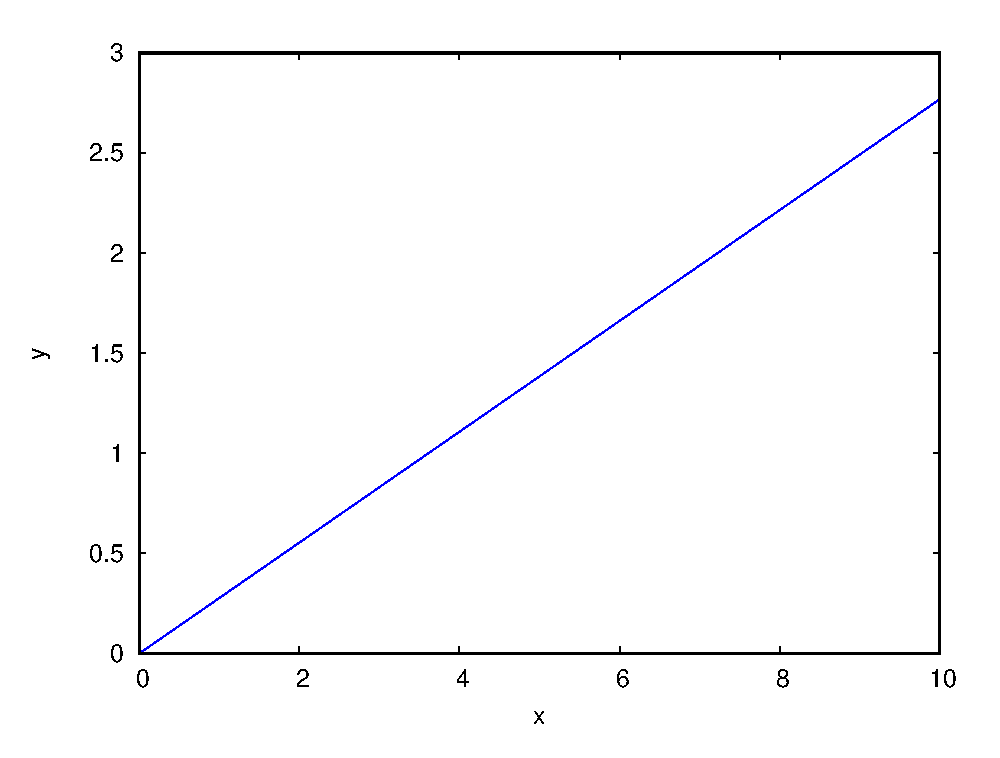
\includegraphics[width=\linewidth, height=30mm]{pic/_sol__0_0_1__0__10__1e2_theta}
    %     \caption{$\theta(t)$}
    %     \label{fig:_sol__0_0_1__0__10__1e2_theta}
    % \end{subfigure}
    % \vspace{12pt}
    
    % \begin{subfigure}[t]{0.3\textwidth}
    %     \centering
    %     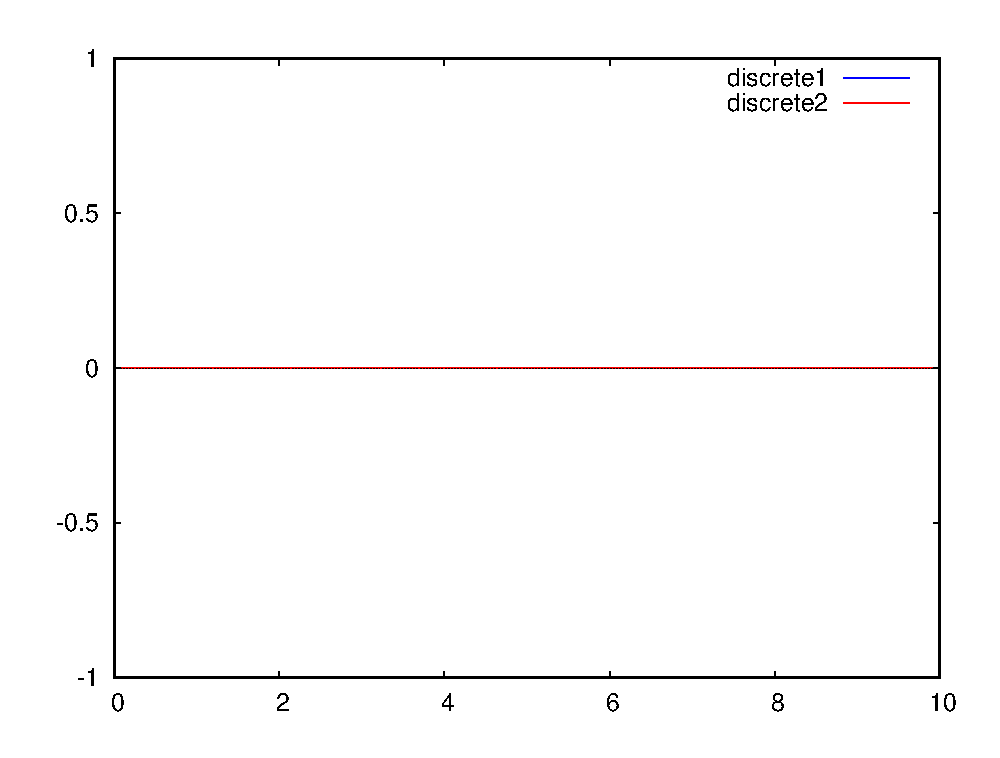
\includegraphics[width=\linewidth, height=30mm]{pic/_sol__0_0_1__0__10__1e2_nu12}
    %     \caption{$\nu_1(t), \nu_2(t)$}
    %     \label{fig:_sol__0_0_1__0__10__1e2_nu12}    
    % \end{subfigure}
    % \hfill
    % \begin{subfigure}[t]{0.3\textwidth}
    %     \centering
    %     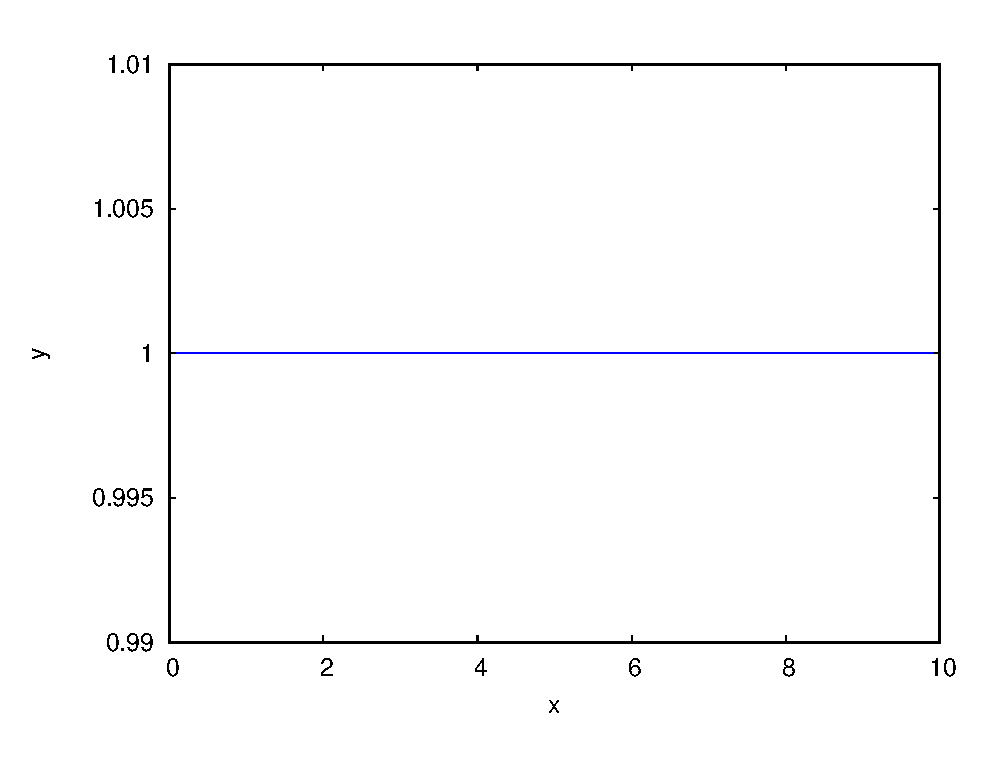
\includegraphics[width=\linewidth, height=30mm]{pic/_sol__0_0_1__0__10__1e2_nu3} \\
    %     \caption{$\nu_3(t)$}
    %     \label{fig:_sol__0_0_1__0__10__1e2_nu3}
    % \end{subfigure}
    % \hfill
    % \begin{subfigure}[t]{0.3\textwidth}
    %     \centering
    %     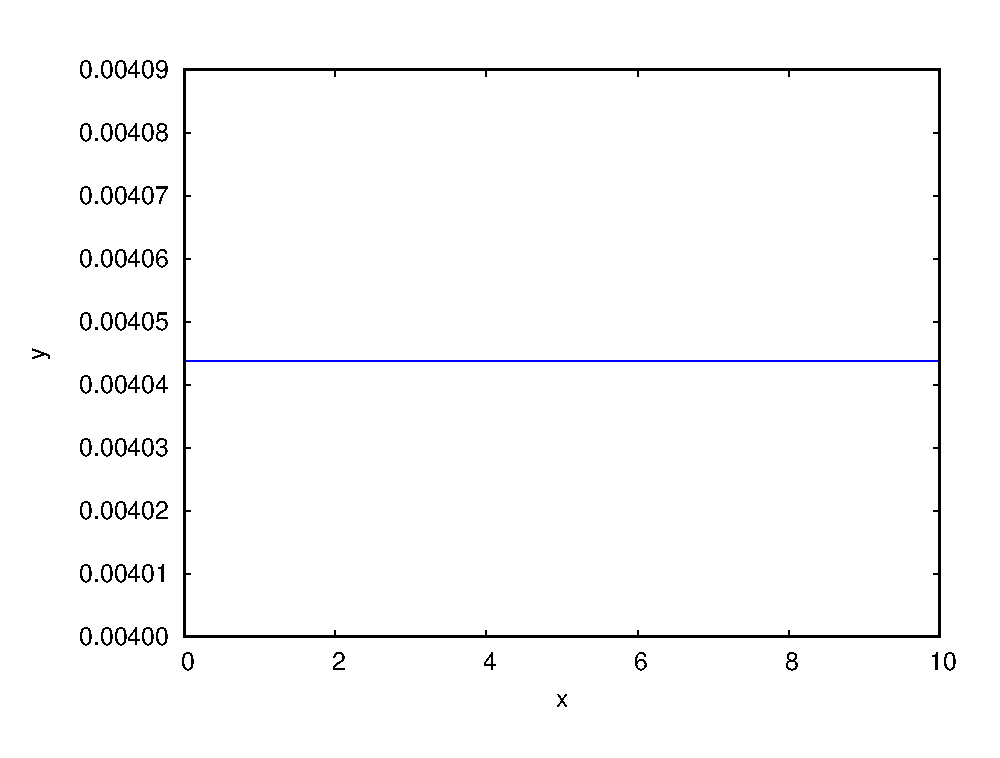
\includegraphics[width=\linewidth, height=30mm]{pic/_sol__0_0_1__0__10__1e2_kin_en}
    %     \caption{Кинетическая энергия}
    %     \label{fig:_sol__0_0_1__0__10__1e2_kin_en}
    % \end{subfigure}
    
    \begin{subfigure}[t]{0.3\textwidth}
        \centering
        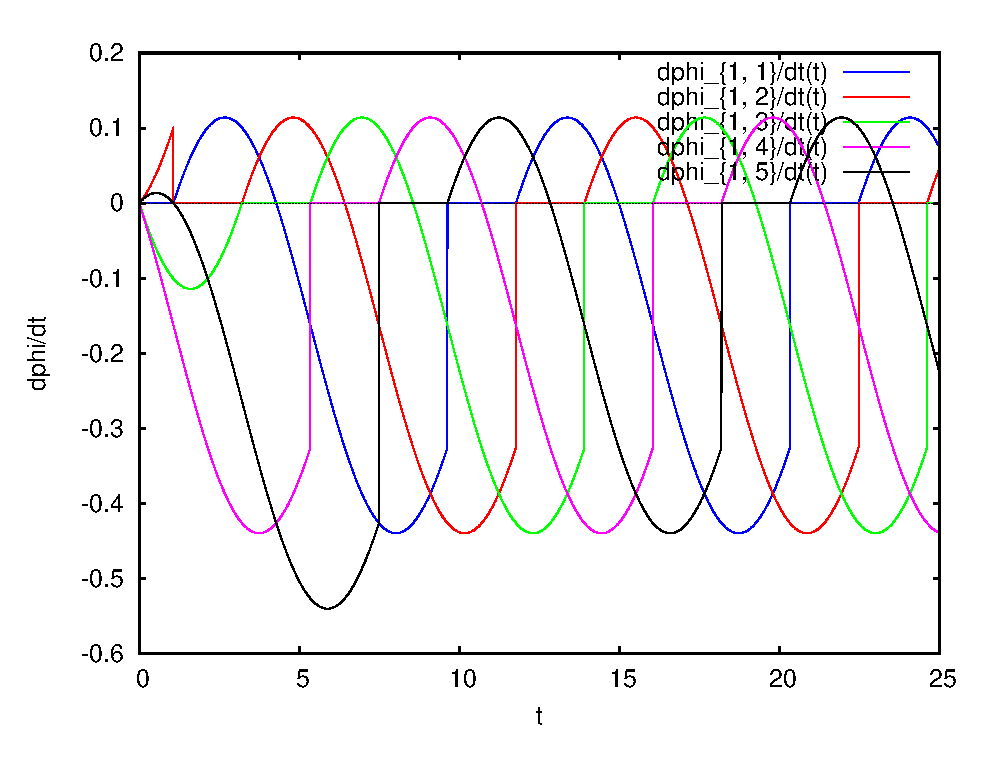
\includegraphics[width=\linewidth]{pic/rol__self_rot__velocities_of_rollers_of_wheel_1}
        \caption{Скорости роликов $\dot{\phi}_{ij}(t)$ на любом колесе}
        \label{fig:rol__self_rot__velocities_of_rollers_of_wheel_1}
    \end{subfigure}
    \begin{subfigure}[t]{0.3\textwidth}
        \centering
        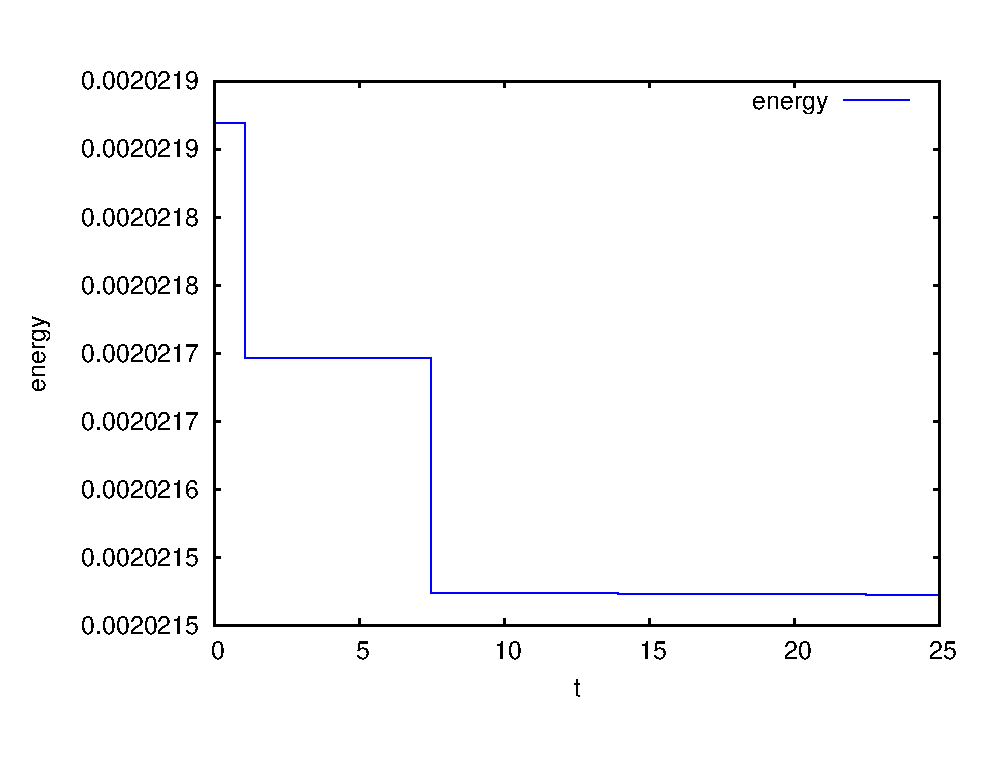
\includegraphics[width=\linewidth]{pic/rol__self_rot__kinetic_energy}
        \caption{Кинетическая энергия}
        \label{fig:rol__self_rot__kinetic_energy}    
    \end{subfigure}
    \begin{subfigure}[t]{0.3\textwidth}
        \centering
        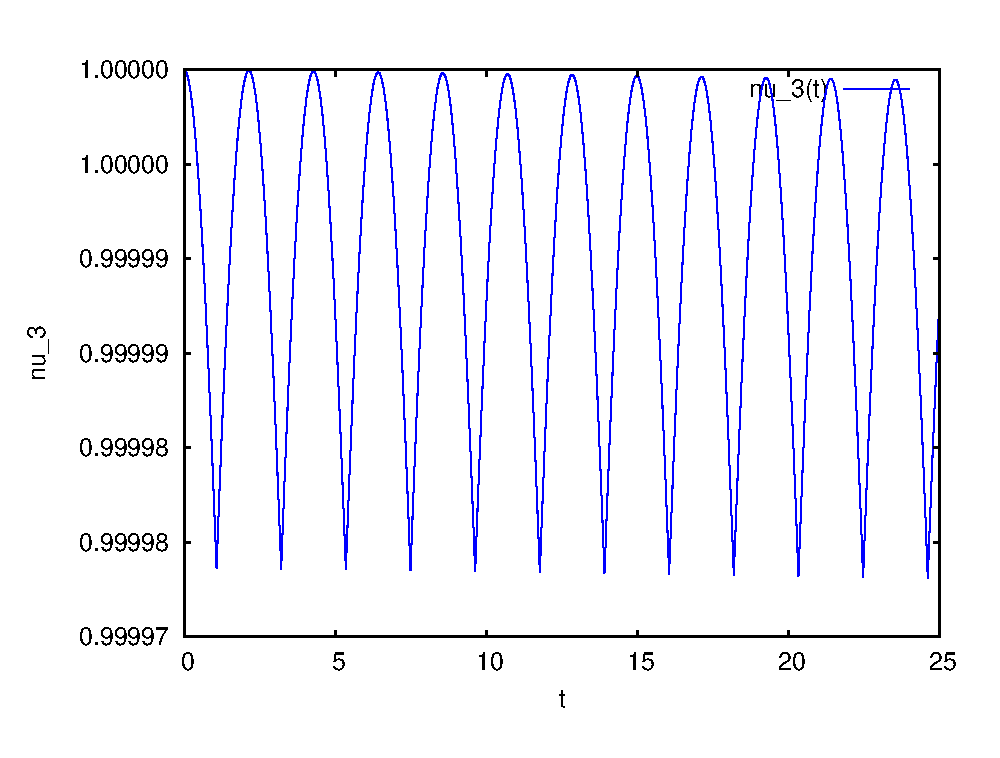
\includegraphics[width=\linewidth]{pic/rol__self_rot__velocity_of_self_rotation}
        \caption{Угловая скорость собственного вращения $\nu_3(t)$}
        \label{fig:rol__self_rot__velocity_of_self_rotation}    
    \end{subfigure}

    \caption{Экипаж с роликами. Вращение вокруг своей оси ($\nu_{1,2}(0) = 0, \nu_3 = 1$).}
    \label{fig:selfrot}
    
\end{figure}


%\begin{figure}[H]
    \centering

    \begin{columns}
        \column{0.45\textwidth}
            \centering
            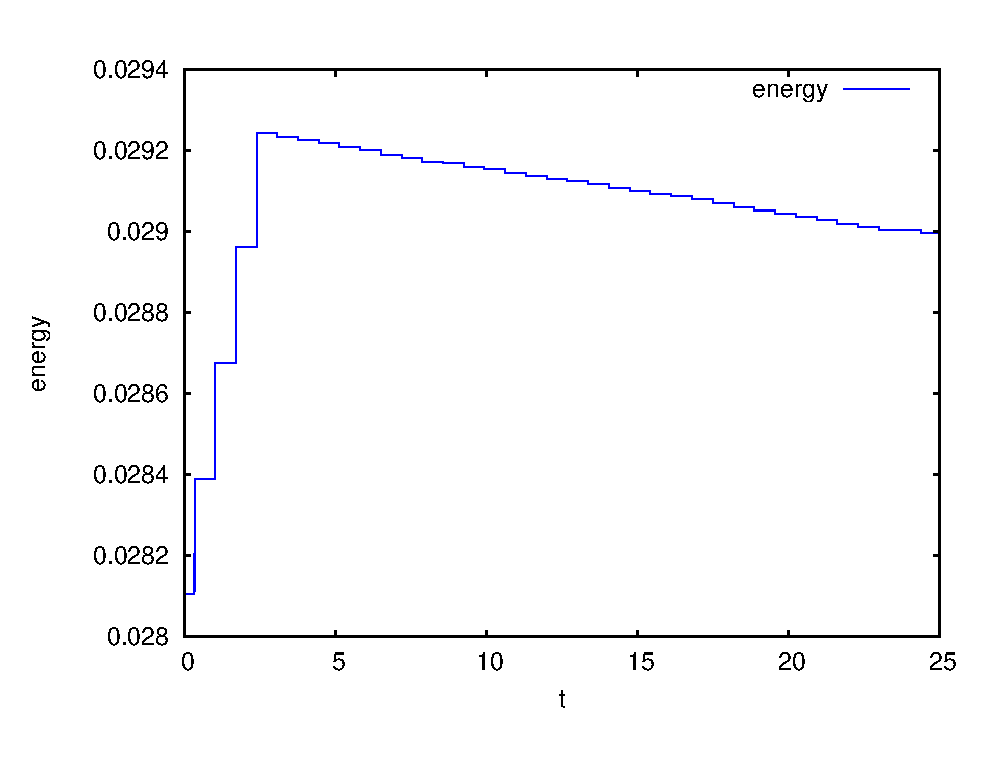
\includegraphics[width=\linewidth]{pic/rol__straight__kinetic_energy}\\
            Кинетическая энергия
        \column{0.45\textwidth}
            \centering
            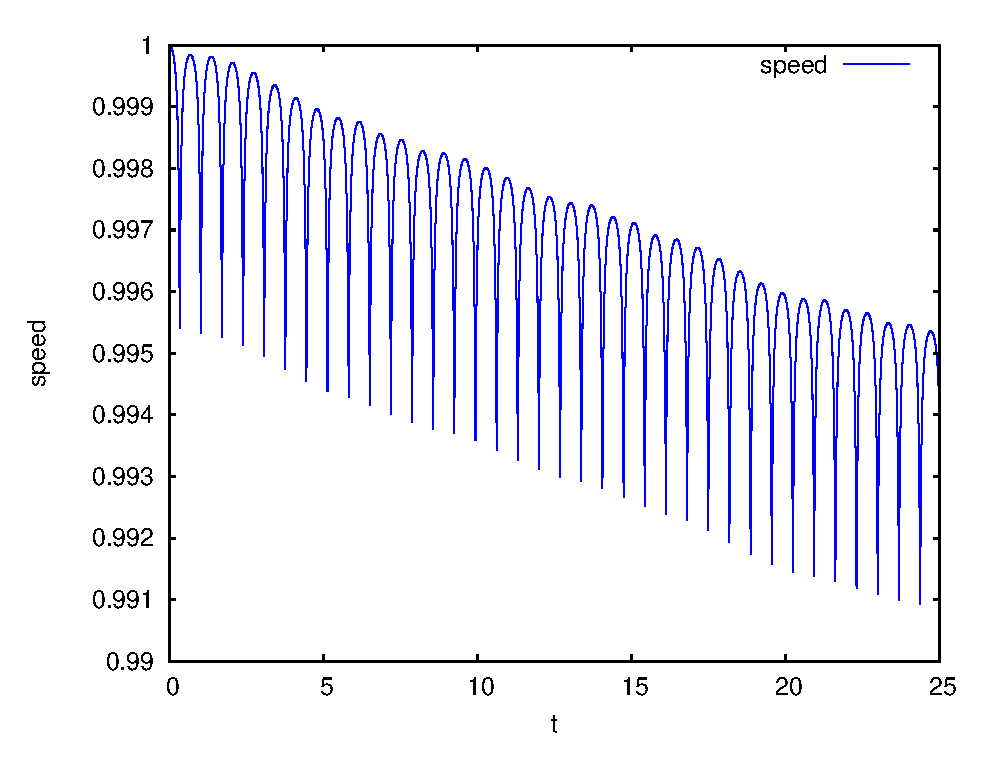
\includegraphics[width=\linewidth]{pic/rol__straight__speed_of_center_of_mass}\\
            Скорость центра масс
    \end{columns}
    
    \begin{columns}
        \column{0.35\textwidth}
            \centering
            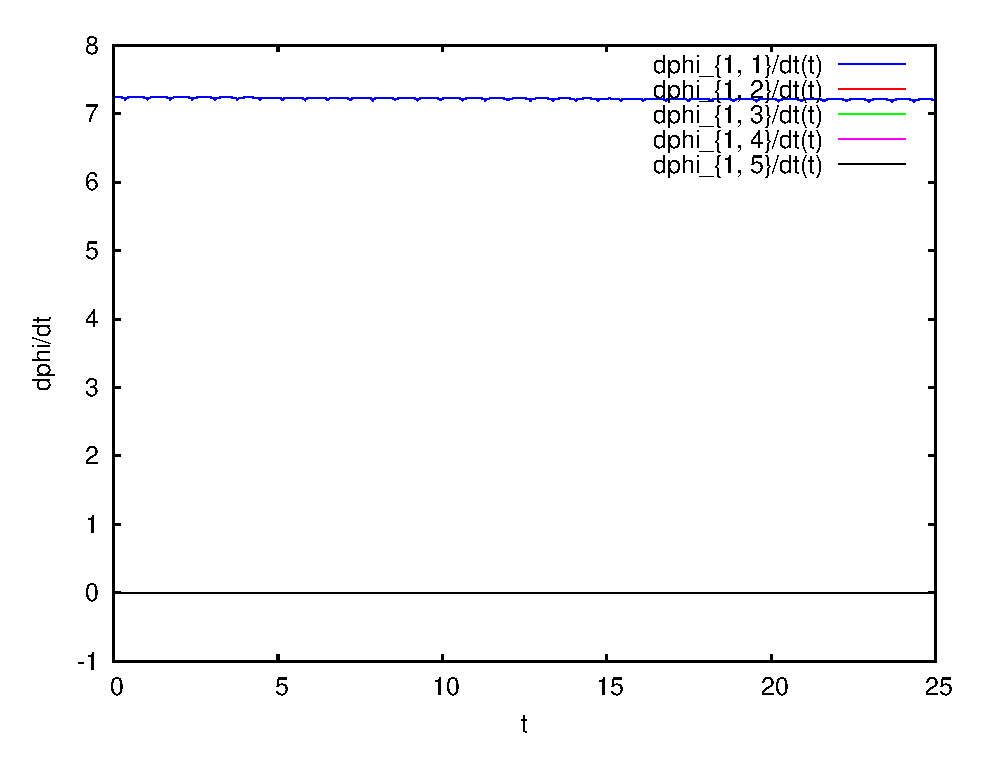
\includegraphics[width=\linewidth]{pic/rol__straight__velocities_of_rollers_of_wheel_1}\\
            $\dot{\phi}_{ij}(t)$ на переднем колесе
        \column{0.45\textwidth}
            \centering
            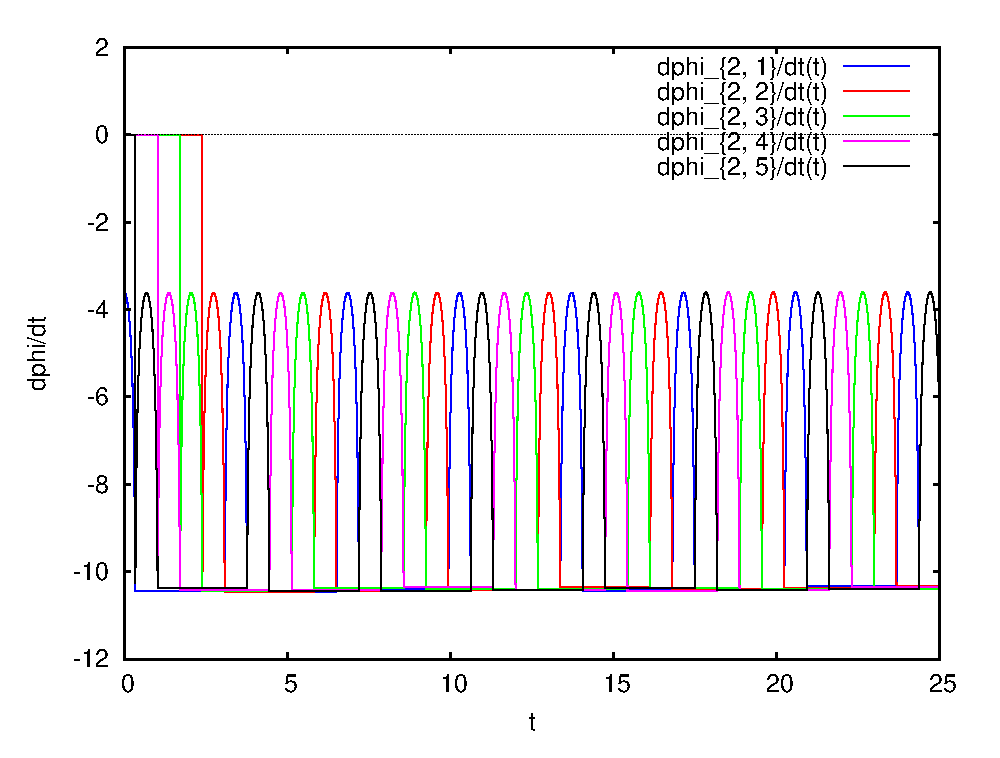
\includegraphics[width=\linewidth]{pic/rol__straight__velocities_of_rollers_of_wheel_2}\\
            $\dot{\phi}_{ij}(t)$ на правом заднем колесе
    \end{columns}

\end{figure}


%\begin{figure}
    \centering
    \begin{subfigure}[t]{0.45\textwidth}
        \centering
        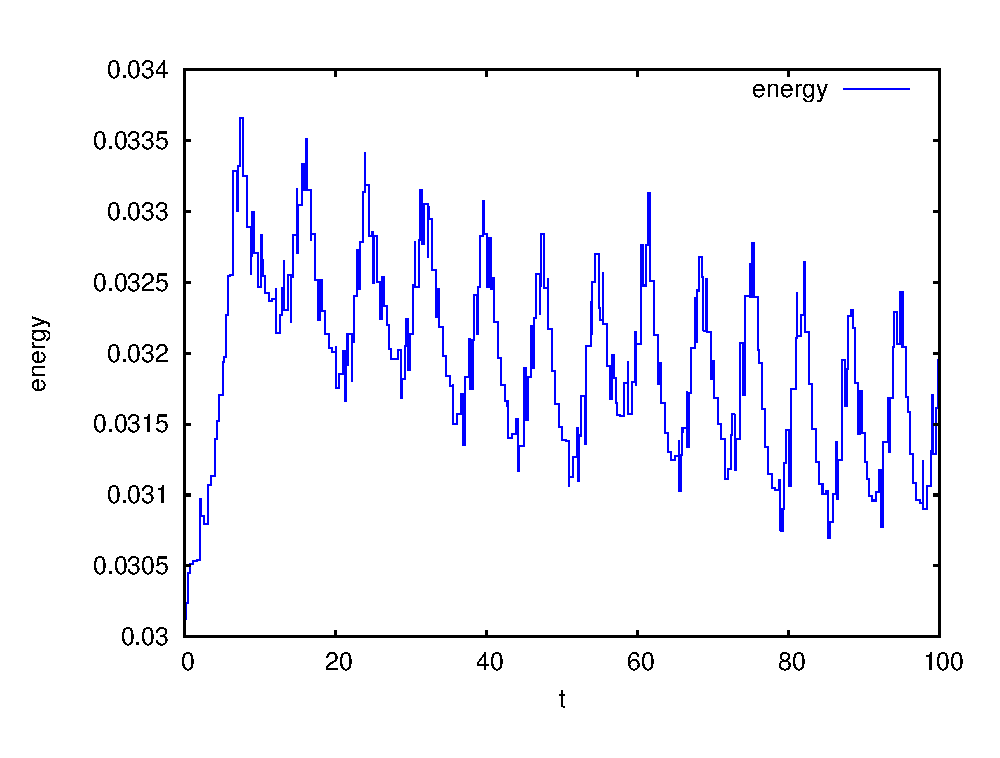
\includegraphics[width=\linewidth]{pic/rol__wrench__kinetic_energy}
        \caption{Кинетическая энергия}
        \label{fig:rol__wrench__kinetic_energy}
    \end{subfigure}
    \begin{subfigure}[t]{0.45\textwidth}
        \centering
        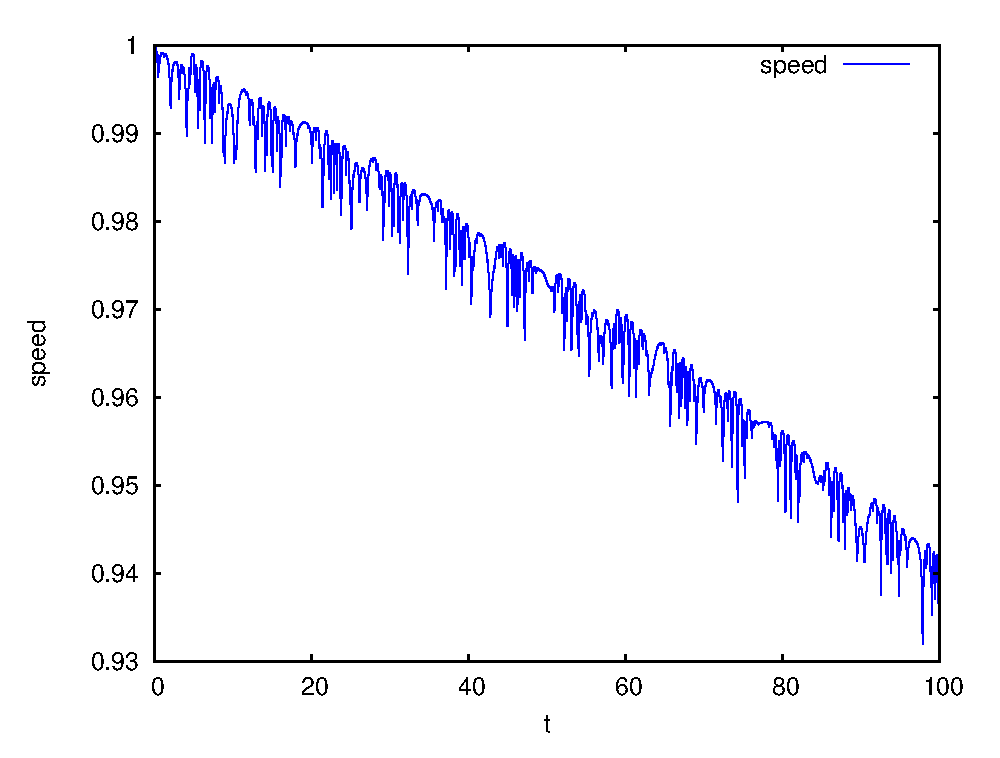
\includegraphics[width=\linewidth]{pic/rol__wrench__speed_of_center_of_mass}
        \caption{Скорость центра масс $\left(\nu_1^2 + \nu_2^2\right)(t)$}
        \label{fig:rol__wrench__speed_of_center_of_mass}
    \end{subfigure}
    \vspace{12pt}
    
    \begin{subfigure}[t]{0.45\textwidth}
        \centering
        \includegraphics[width=\linewidth]{pic/rol__wrench__velocities_of_rollers_of_wheel_1}
        \caption{Скорости роликов $\dot{\phi}_{ij}(t)$ на первом колесе}
        \label{fig:rol__wrench__velocities_of_rollers_of_wheel_1}    
    \end{subfigure}
    \hfill
    \begin{subfigure}[t]{0.45\textwidth}
        \centering
        \includegraphics[width=\linewidth]{pic/rol__wrench__trajectory} \\
        \caption{Траектория центра масс на плоскости $OXY$}
        \label{fig:rol__wrench__trajectory}
    \end{subfigure}
    
    \caption{Экипаж c роликами. Движение с закруткой ($\nu_1(0) = 1, \nu_2(0) = 0, \nu_3(0) = 1$).}
    \label{fig:wrench}
    
\end{figure}


%\newpage

%\section{Приложение}

%\appendix

% {\bf Авторы.}

\begin{itemize}
    \item Герасимов Кирилл Вячеславович (Kirill Gerasimov); 119234, Москва, Ленинские горы, 1Б, 1725; 8 (925) 033-60-79; kiriger@gmail.com;
    \item Зобова Александра Александровна (Alexandra Zobova); Москва, Дмитровское шоссе, 165Е, корп. 1, кв. 28; 8 (916) 333-19-78; azobova@mech.math.msu.su.
\end{itemize}
    
    Кафедра теоретической механики и мехатроники механико-математического факультета МГУ им. М.В. Ломоносова, Москва, Тел.: (495) 939-36-81
    
    On the motion of a symmetrical vehicle with omniwheels with massive rollers
    

\newpage
\begin{center}
\large
\textbf{ ON THE MOTION OF A SYMMETRICAL VEHICLE WITH OMNIWHEELS WITH MASSIVE ROLLERS \\
\textcopyright \ 2018 г. \quad K. Gerasimov$^{1,*}$, A. Zobova$^{1,**}$ }

\textit{ $^1$ Chair of Theoretical Mechanics and Mechatronics, Department of Mechanics and Mathematics, Lomonosov Moscow State University \\
$^*$E-mail: kiriger@gmail.com, $^{**}$E-mail: azobova@mech.math.msu.su }
\end{center}

\end{document}


